\documentclass[12pt,letterpaper,oneside]{book}

\usepackage{afitStyleFiles/afitThesis}
\usepackage{afitStyleFiles/sf298}
\usepackage[acronym, toc,shortcuts]{glossaries}
\usepackage{algorithm}
\usepackage{algpseudocode}
\usepackage{bm}
\usepackage[table,xcdraw]{xcolor}
\usepackage{listings}
\usepackage{silence} \WarningFilter{fixltx2e}{}
\usepackage{stringstrings}
\usepackage{titlecaps}
\usepackage{cleveref} % for \Cref, etc.
\usepackage{textcomp}
\usepackage{siunitx} % for using scientific notation for numbers, can include units easily and "x10^6" etc.
\usepackage[section]{placeins}
\lstset{basicstyle=\ttfamily,breaklines=true}
\sisetup{
	round-mode          = places, % Rounds numbers
	round-precision     = 3, % to 2 places
	per-mode=symbol,
	% fraction-function=\sfrac % for different style of fractions
}

% KJ Nelson added to afitThesis.sty:
%\usepackage[hyphens]{url}
%\usepackage{hyperref}


% Include paths for image files
\graphicspath{{figures/}}
\usepackage{subcaption}
%% Customize your document with your personal information
%% First, comment out the appropriate document type
\afitthesis %%default
% \afitreport
% \dissertation
% \prospectus

\author{Matthew M. Rofrano, B.S.E.E.}
\rank{Captain, USAF} % If a civilian, comment out this line.

\docdesignator{AFIT-ENG-MS-20-M-XXX} % Update from list from
\department{Department of Electrical and Computer Engineering}
\graduationdate{March 24, 2023}

\flytitle{Classifying Open-Air Target Measurements via Simulation-Trained Convolutional Neural Networks }
\title{Classifying Open-Air Target Measurements via Simulation Trained Convolutional Neural Networks }
                             % Note, if you use \MakeUppercase to put
                             % the title in all uppercase as the style
                             % guide demands, understand that the
                             % command does not allow page breaks ``\\''
                             % within its brackets.
\previousdegrees{B.S.E.E.}
\acdegree{Master of Science in Electrical Engineering}

\committee{{Robert F. Mills, Ph.D\\Chair},
           {Charles XX. Macon,, Ph.D\\Member},
           {DUNNO-SOME LO DUDE,, Ph.D\\Member}}

\address{2950 Hobson Way\\ Air Force Institute of Technology \\
Wright-Patterson AFB, OH 45433}

\distribution{DISTRIBUTION STATEMENT A\\[-10pt]
\MakeUppercase{Approved for Public Release; distribution unlimited.}
}

\disclaimer{The views expressed in this document are those of the
author and do not reflect the official policy or position of the
United States Air Force, the United States Department of Defense or
the United States Government.  This material is declared a work of the
U.S. Government and is not subject to copyright protection in the
United States.}

% International students may consider using the following disclaimer
% statement: \dislaimer{The views expressed in this document are those
% of the author(s) and do not reflect the official policy or position
% of the United States Air Force, Department of Defense, United States
% Government, the corresponding agencies of any other government,
% NATO, or any other defense organization.}

\makenoidxglossaries
\loadglsentries{myThesis/glossary}




\begin{document}
%\glossaryAcronyms
{\frontmatter
\flyleaf
\disclaimerpage
\titlepageAFIT
\committeepage  }
\phantomsection
\begin{abstract}	
	
Abstract text here. Put in acronyms, like \gls{UAV}. Or cite items like with \cite{Scaramuzza2011} in a bibtex file auto-updated from Mendeley.
	

\end{abstract}

\phantomsection %not sure exactly what this does, but it helps with Table of Contents and References
{
\tableofcontents
\glsunsetall % resets all acronyms, so all will be spelled out again
\listoffigures
\listoftables
% UNUSED
%\listofabbreviations
%\listofsymbols

\mainmatter }
\phantomsection
\chapter{Introduction}
\label{ch:introduction}
\glsresetall

\section{Problem Background}
\label{ch:problem_statement}

The Department of Defense Electromagnetic Spectrum Superiority Strategy states clearly that the Electromagnetic spectrum is a battleground, inseparable from the classical settings of war. The expectation for future near-peer conflict will result in a highly `congested, contested, and constrained Electromagnetic Operating Environment (EMOE) \cite{DOD_ESSS}' The DoD EMSSS seeks to develop equipment that will be flexible, efficient, resilient. This project seeks to support this vision for the future EMS war by examining tactics that create congestion and confusion in the EMOE. Particularly, the employment of air borne platforms.

Decoy airborne platforms were conceptualized as early as 1952, with the development and test of the XSM-73 `Goose' ground-launched airborne decoy which was later reconfigured as an air-launched platform, and re-designated the ADM-20 `Quail'. The Quails' purpose was to overwhelm an adversary integrated air-defense system (IADS), allowing for bomber and strike aircraft to penetrate the airspace and prosecute targets. The Quail was succeeded by the ADM-141 TALD, or Tactical Air-Launch Decoy which was employed with good effect during the first night of the Gulf War. Launched in coordination with BQM-74 target drones, the decoy platforms were launched towards Baghdad to force a response from adversary IADS. The operation was a success:  adversary radars were forced to engage the unknown targets, which opened them up to attack from Coalition Anti-Radiation missiles. There was an additional benefit of forcing attrition on the Iraqi Air Defense's Surface to Air missile stores:  the cheaply produced decoys were an effective sponge for the more costly surface to air missiles.

Airborne decoys play a specific role in the contested EMOE:  they degrade the air defenders view of the scene; force radars to engage the decoys, exposing themselves to anti-radiation fires; and force engagement, which depletes the IADS available surface to air missile stores.

The power of decoy missiles is that on physical inspection they appear similar in shape size, and speed to their lethal relatives. An example is shown in figure \ref{fig:missiles}, where an air-launched decoy is set alongside its potentially nuclear-equipped cousin.

\begin{figure}[htbp]
  \centering
  \begin{subfigure}{.5\textwidth}
    \centering
    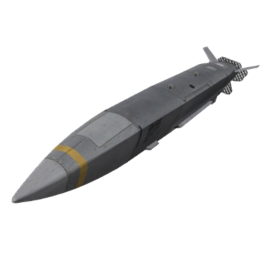
\includegraphics[width=.8\linewidth]{adm-160.png}
  \end{subfigure}%
  \begin{subfigure}{.5\textwidth}
    \centering
    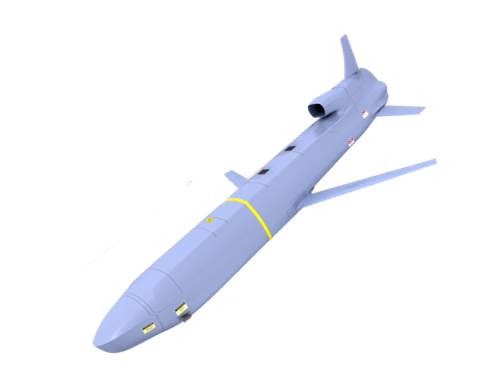
\includegraphics[width=.8\linewidth]{agm-86.png}
  \end{subfigure}
  \caption[Air Launched Platform Comparison]{An ADM-160B MALD and AGM-86 Air Launched Cruise Missile (ALCM)}
  \label{fig:missiles}
\end{figure}


This paper seeks to a solution to this problem:  a hypothetical sensor with an embedded machine learning model is trained to classify similar targets using radar cross section data. This project accepts the likelihood that the true RCS data for an adversary target would not be available, and instead utilizes simulation data to train the model. The models performance is tested using measurement data taken from an open-air range.


\section{Research Objectives}
\label{sec:objectives}

The principle goals of this project are to analyze and document the performance of a machine learning network's ability to classify targets. The model will be trained using simulation data, and evaluated using measured data. Additionally, this paper will document data normalization techniques for RCS data; quantify sensor performance breakdowns in terms of signal correlation; as well as document performance enhancing techniques such as multi-model comparators, and multi-angle training.

\section{Document Overview}
\label{sec:overview}

Chapter 2 of this document cover background information relevant to this project: radar operation, electromagnetic waves and target interaction, as well as a review of similar projects and the current state of machine learning models in signal processing. Chapter 3 will outline the methodology employed in this experiment to include data collection for both simulated and measured targets; measurement calibration; data augmentation, and model evaluation. Chapter 4 will report the experiments findings, and chapter 5 will present a conclusion

\phantomsection
measuring\chapter{Background and Literature Review}
\label{ch:background}
\glsresetall

\section{Overview}

An overview of the this project is presented in figure \ref{fig:overview}. \gls{RCS} is collected from open air measurement, and simulation. Collected data is modified using \gls{AWGN} to create both training and test datasets. Datasets are augmented, and passed to a machine learning model that will classify the targets as one of five potential targets. Training data will be used to determine optimal model parameters, and test data will be used to quantify accuracy. This conception: simulation data for training, measured data for evaluation is referred to as a `model based approach'. The primary performance measurements will be a confusion matrix, as well as a correlation matrix. The confusion matrix documents the models predictions, and whether they are correct or incorrect. The cross correlation matrix documents the `similarity' between the targets RCS measurements, and will be the primary tool for understanding success or failure in classification accuracy.

\begin{figure}[htbp]
	\centering
	 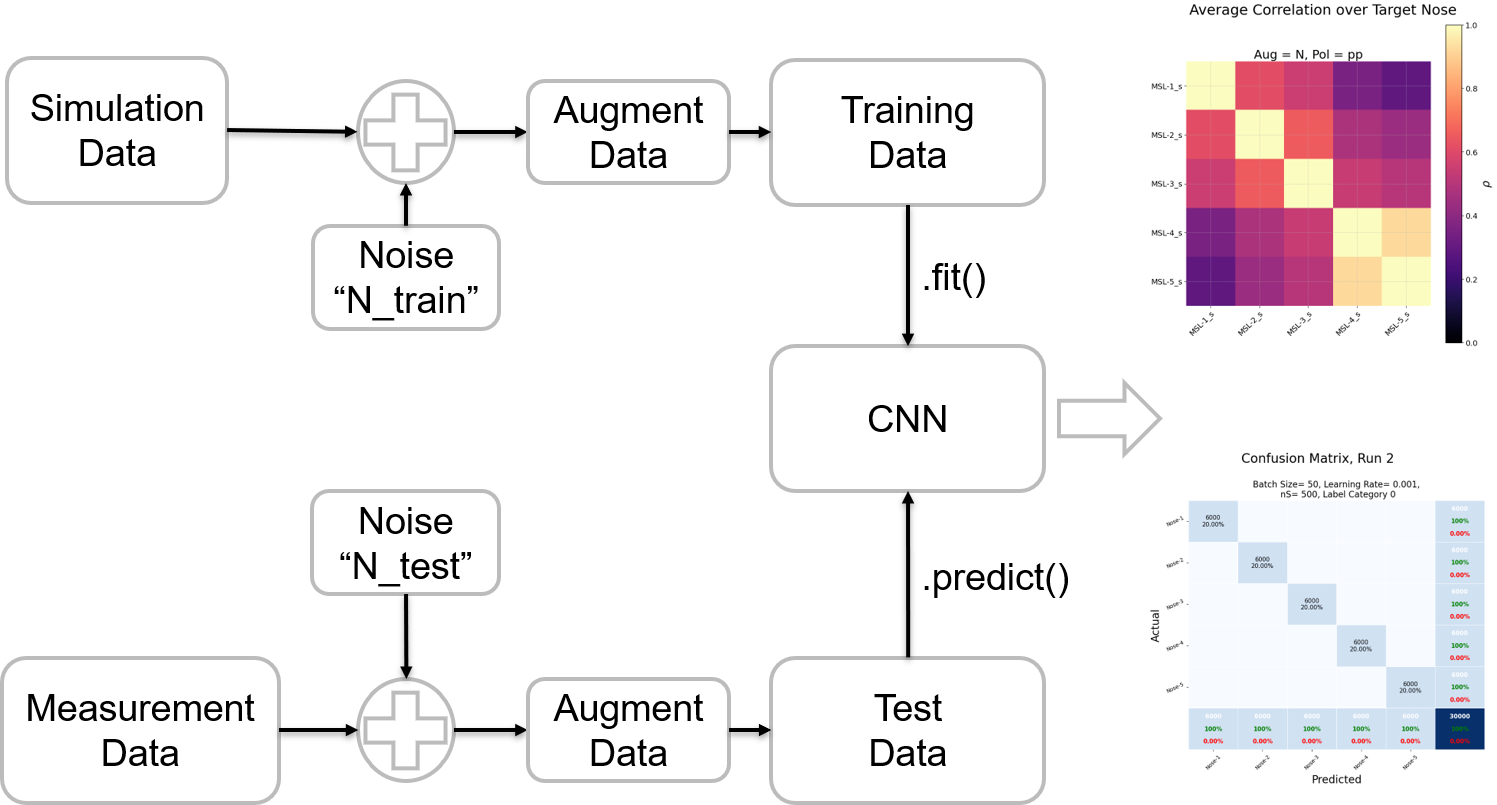
\includegraphics[width=.8\linewidth]{flow_chart.png}
	\caption[Project Overview]{Project overview flow chart.}
	\label{fig:overview}
\end{figure}

\section{Simulation and Measurement Data}

The simulation and measurement data used for project is captured/simulated using the reaction of metallic targets in the presence of electromagnetic fields. These fields are typically launched from a radar system, whose high transmission power and sensitive receiver allow the system to identify potential targets at long range. A radars theoretical performance can be quantified using the radar range equation, which incorporates the radars transmission power, sensitivity, as well as the target radar cross section. The omnipresence of noise degrades a radar's ability to detect targets. The radar's \gls{SNR} performance is a figure of merit that documents a radars capabilities in the presence of natural, or adversarial noise. The following sections will detail the phenomena listed above, as well as document how they will be employed throughout this project.

	\subsection{Electromagnetic Wave Interaction}
	\label{sec:EM}

		\gls{EMR} as used by wireless systems is produced by the time-varying motion of charge. The mathematical model for EMR arises from solutions to Ampere's law with Maxwell's addition

		\begin{align}
			\nabla \times \vec{B} &= \frac{\partial}{\partial t} \mu \epsilon \vec{E} + \mu \vec{J} \label{eq:AMP}.
		\end{align}

		Here, $\vec{B}$ and $\vec{E}$ are the magnetic flux density and Electric Field strength respectively. The term $\vec{J}$ represent source current, and is equal to zero in free space. The \textit{intrinsic properties} $\mu$ and $\epsilon$ represent the magnetic permeability and electrical permeance of the material the fields are interacting with. These are the \textit{constitutive relations} that link the interaction of a field with the physical world \cite{KONG}.

		Ampere's law is a second order differential equation. When source current is equal to zero, it can be rearranged to take the form of the Helmholtz wave equation:

		\begin{align}
			\nabla^2 \vec E - \mu \epsilon \vec{E} = 0 \label{eq:helm_wave}.
		\end{align}

		Solutions to the Helmholtz wave equation that satisfy Maxwell's laws are \gls{EM} \cite{KONG}. Assuming an EM wave polarized in the $\hat{x}$ axis and propagating in the $z$ direction, a solution would take the form:

		\begin{align}\label{eq:wave_sol}
			\nabla^2 \vec E   = \mu \epsilon \vec{E} \notag\\
			\vec{E} = \hat{x}E_0\cdot \cos(kz - \omega t).
		\end{align}

		The term $k$ is the dispersion relation $\omega\sqrt{\mu_0 \epsilon_0}$, and $\omega$ is the frequency of oscillation for the time-varying signal displacement current.

		The solution provided by equation \ref{eq:wave_sol} is useful for analyzing a waves interaction with material in free space. This wave will interact with any material whose intrinsic properties differ from the wave's dispersion relation. These regions are called \textit{boundaries}, and demarcate a change in the intrinsic properties of the medium as seen by the wave. This paper will focus on the interaction of a wave in air as it meets a \gls{PEC}. A PEC is any material whose intrinsic properties make it appear to be a perfect conductor. The energy of the propagating wave, incident on a PEC wave will be completely converted to a surface current. This surface current produces a reflection of the incident wave \cite{KONG}. The reflection produced by the boundary in the presence of incident EMR is what allows radars to operate. Assuming the reflections are sufficiently powerful, a detector can capture them and infer information about the target.

	\subsection{Radar}
		\label{sec:RD}
	 	The first \gls{RADAR} device was patented by German inventor Christian H{\"u}lsmeyer. Serving as a means to help ships avoid collision in heavy fog, radar showed impressive all weather long distance performance. This initial concept was expanded on by a British meteorologist named Robert Watson-Watt. Watt measured the EMR from lighting bursts using an oscilloscope as a means to track storms. Watt's innovation was using an oscilloscope to display the signals, which improved received signal fidelity compared to the H{\"u}lsmeyer detector. The British Air Ministry, sensing an impending war with Germany quickly pressed to militarize Watt's invention. In November 1934 the Committee for the Scientific Survey of Air Defense convened. Watt and his assistant Arnold `Skip' Wilson proposed a radar system that could not only detect enemy aircraft, but could determine their range as well. The first operational pulse radar detected a Supermarine Scapa flying boat at a distance of 17 miles on 17 June 1935, ushering in the era of air defense radars in modern warfare \cite{Bowen}.

		Radar performance is commonly quantified using the radar range equation (RRE). The RRE is an extension of the radiation field solution using a far-field approximation \cite{KONG}, given by

		\begin{equation}\label{eq:re}
			P_{r} = \frac{P_t}{4 \pi R_{r, t}^2}G_t \cdot \frac{\sigma(\theta, \phi)}{4 \pi R_{t, r}^2} \cdot \frac{G_r \lambda^2}{4 \pi}
		\end{equation}

		where  ($\frac{P_t }{4 \pi R_{r, t}^2}G_t$) represents the transmitted signal power density attenuated over distance $R_{r, t}$ from the radar to the target; ($\frac{\sigma}{4 \pi R^2}$) represents target interaction, echo emission, and echo attenuation over distance $R_{t, r}$; and ($\frac{G_r \lambda^2}{4 \pi}$) models receiver gain and sensitivity. \cite{POMR_Range_eq}.

		The terms $P_t$ and $P_r$ represent the transmitted power of the initial signal, and the received echo signal respectively. The gain terms $G_t$ and $G_r$ represent the directionality of the transmit and receive antennas respectively, and are equivalent for a mono-static radar configuration. A mono-static radar utilizes a single antenna to both transmit and receive signals.

		Target interaction leverages the behavior of electromagnetic waves at boundaries as discussed in section \ref{sec:EM}. A metallic, or PEC target will re-emit an echo signal with a directional intensity given by its RCS pattern, $\sigma(\theta, \phi)$. The response of $\sigma$ is primarily driven by the physical shape of the target. A principle of low-observable design seeks to control $\sigma$ by directing scattered pulses away from the mono-static radar.

		The receiver term shows a dependence on frequency for $\lambda = c/f$, where $c = 3\times 10^8 [m/s]$, and $f$ is the carrier frequency of the transmitted signal. This frequency dependence is driven by antenna design. Antennas have an optimal shape that is tailored to their operating frequency band. The antennas used for this experiment are within their operating bands for all frequencies. However, this frequency dependence will play an important role in equipment calibration, which will be discussed in section \ref{sec:cal}.

		\section{Measurement Calibration}
	    \label{sec:cal}
	    Open air measurements must account for two distinct error sources:  range intrusion, and instrument calibration. Range intrusion accounts for spurious echo's from the floor, walls, target mount, and other physical objects in the range that interact with the incident field. These signals constitute the `background' of the scene and can be mitigated in two ways:  1. gating returns at the receiver to create quiet zones; 2. Implementing background subtraction using

	    \begin{equation}
	      E_{t, true} = E_{t, raw} - E_{t, bg}
	    \end{equation}

	    where $E_{t, raw}$ and $E_{t, bg}$ are measurements of the scene with and without the target in place. While background subtraction will help to reduce spurious signals, it cannot account for target-mount interactions and will not completely eliminate spurious returns.

	    The instrument radar is calibrated using the substitution method:  a simple target whose RCS can be readily calculated is used to create a proportionality constant which accounts for deviations in radar performance \cite{Knott}. Since the range distances are fixed, the only factor of the radar range equation that will change is either the target's RCS, or fluctuation in transmitted power over frequency. By measuring a target with a known RCS, the proportionality constant $C$ can determined using

	    \begin{equation}
	      C = \frac{E_{cal, sim}}{E_{cal, raw} - E_{cal, bg}}
	    \end{equation}

	    where $E_{cal, raw}$ and $E_{cal, bg}$ are measurements of the scene with and without the calibration target respectively. The term $E_{cal, sim}$ is the RCS measurement of the calibration target. This experiment utilizes a 7 inch calibration cylinder whose RCS is modeled using CADFeko. Notably, the substitution method employs background subtraction as discussed previously.

	    Prior to data processing, all target measurements are calibrated using

	    \begin{equation}
	      E_{t, true} = \frac{E_{t, raw} - E_{t, bg}}{E_{cal, raw} - E_{cal, bg}}
	    \end{equation}

		\section{Instrumentation Quiet Zone}
			An instrumentation radar can be configured to exclude radar echoes that are outside of a desired location. This is desirable when collecting data. The receiver of the radar is \textit{gated}, or configured in a manner to only `listen` for echoes during a certain window. The windows are configured in temporal time. Due to the speed of light, these temporal time values directly correspond with a location using

			\begin{equation}
				d = \frac{c \times \Delta t}{2}
			\end{equation}

			where $d$ is a distance in meters, $c$ is the speed of light in $m/s$ and $\Delta t$ is elapsed time. This equation is divided by 2 due to the two-way path a radar pulse must travel. As an example, a preferred quiet zone that begins 5 meters from the radar, and ends  10 meters from the target would have a reception time window between $33.3$ and $66.7$ nano seconds.

\section{Signal to Noise Performance}

	A radars operational `field of view' is limited by the sensitivity of its receiver. Field of view in this context refers to the distance and azimuth over which the radar can successfully identify and prosecute targets. Sensitivity measures the minimum signal level that the radar can detect. If a signal is too faint, it will fall below the noise floor of the system  and become irrecoverable.

	The noise floor defines the power level, $P_n$ below which received signals will be lost. Typically, the noise floor is driven by the thermal noise of the radars receiver. Thermal noise current accounts for the random fluctuations of moving charges in matter above 0K and can functionally defined as

	\begin{equation}\label{eq:tnoise}
		P_n = k_B T_S B = k_B T_0 F B
	\end{equation}

	Where $k_B$ is Boltzmann's constant \footnote{$1.38\times10^{-23} W\cdot s / K$}, $T_S$ is the system temperature in Kelvin, $B$ is the instantaneous receiver bandwidth in Hz, $T_0$ is the standard temperature \footnote{$T_0 = 290 K$}, and $F$ is the noise figure of the receiver subsystem. System bandwidth is typically driven by the signal the radar emits, and cannot be made arbitrarily small. A radar pulse of length $\tau$ will require a bandwidth of $B = 1/\tau$ \cite{POMR_Noise}\cite{J_Noise}\cite{N_Noise}. A hypothetical system with a noise figure of $F = 1.2$, and bandwidth $B=1$ MHz will have a noise floor of $-112.8$ [dB\_m].

	Thermal noise is modelled as an additive zero-mean gaussian process. Modern radar designs seek to mitigate thermal noise via pulse integration. Adding multiple pulses together reduces noise power since the zero-mean noise tends to zero over multiple integrations. For a coherent system (one in which phase is maintained) the improvement in signal level is directly proportional to $n$, the number of pulses integrated. For a non-coherent system, the integration factor is given as $\sqrt{n}$.

	The radar equation can be re-cast to include thermal noise and the integration factor using

	\begin{equation}\label{eq:re_snr}
		SNR_0 = \frac{P_t}{4 \pi R_{r, t}^2}G_t
		\cdot \frac{\sigma(\theta, \phi)}{4 \pi R_{r, t}^2}
		\cdot \frac{G_r \lambda^2}{4 \pi}
		\cdot \frac{1}{k_B T_S B}
		\cdot n_p
	\end{equation}

	where $SNR_0$ represents the signal to noise ratio of the received signal with respect to the thermal noise in the system. The minimum discernable signal (MDS) of the system is the smallest SNR for which the radar can reliably detect targets in the presence of thermal noise.

	This paper will take measure the SNR as the ratio of the absolute value of phasor RCS data and noise in \gls{dBm}. A milli-watt decibel is the measure of a signal in decibel form, referenced to 1 milli-watt:

	\begin{equation}
		dBm = 10 \times \log(\frac{P [W]}{0.001 [W]})
	\end{equation}

\section{Radar Cross Section}

	RCS is the ratio of scattered to incident power for a given target in the presence of an EM wave. RCS data can be presented in several ways depending on the context, and what information is most relevant. In each of the following cases, data is collected and presented for both vertically and horizontally polarized incident fields. The figures in this section will present horizontally polarized data for expedience.

	An RCS `cut' is a polar plot of RCS data taken at a single measurement frequency over 360 degrees. Total RCS is presented as a contour plot with frequency and angle axes, and magnitude represented by color. The augmentation applied to the data plays an important role in data presentation, since RCS phasor data can have a large dynamic range. Large contributions can be highlighted or suppressed dependent on the augmentation employed. This project will use both plot formats, and several augmentation schemes throughout.

	As an example of plot format, augmentation style, and the behavior of targets in incident field, consider the simulated RCS response of the target shown in figure \ref{fig:msl_target}. The total response, as well as an RCS cut augmented in $m^2$ and $\textrm{db}_{sm}$ are shown in figures \ref{fig:msl_m2}, and \ref{fig:msl_db} respectively.

	The $m^2$ format is calculated using the IEEE definition for RCS,

	\begin{equation}\label{eq:ieee_rcs}
			\sigma [m^2] = 4\pi \frac{|E_{s}|^2}{|E_{i}|^2}
	\end{equation}

	where $E_s$ and $E_i$ are the scattered and incident fields, and $r$ is the distance between the transmitting source and target \ref{eq:ieee_rcs}\cite{Knott}. This data can be re-cast in $\textrm{dB}_{sm}$, or decibel per square meter as follows:

	\begin{equation}\label{eq:ieee_dbsm}
			\sigma [\textrm{db}_{sm}] = 20\times \log\left( \frac{\sigma [m^2]}{1 [m^2]}\right)
	\end{equation}

	The augmentation employed highlights the RCS contribution based on the targets physical construction. In figure \ref{fig:msl_m2} data is presented in $m^2$ format. The specular flash of the cylindrical missile body dominates the return. In figure \ref{fig:msl_db}, the response of the cylindrical body is suppressed, and other RCS contributions can be observed. This project will restrict classification to a sector surrounding the targets nose. Extending $\pm 30^{\circ}$ about the target nose, the sector of interest is shown as a green wedge on the RCS cuts. On the total RCS plots, measurements outside the 60 degree sector are `dimmed.`

	\begin{figure}[htbp]
	  \centering
	  \begin{subfigure}{.5\textwidth}
	    \centering
	    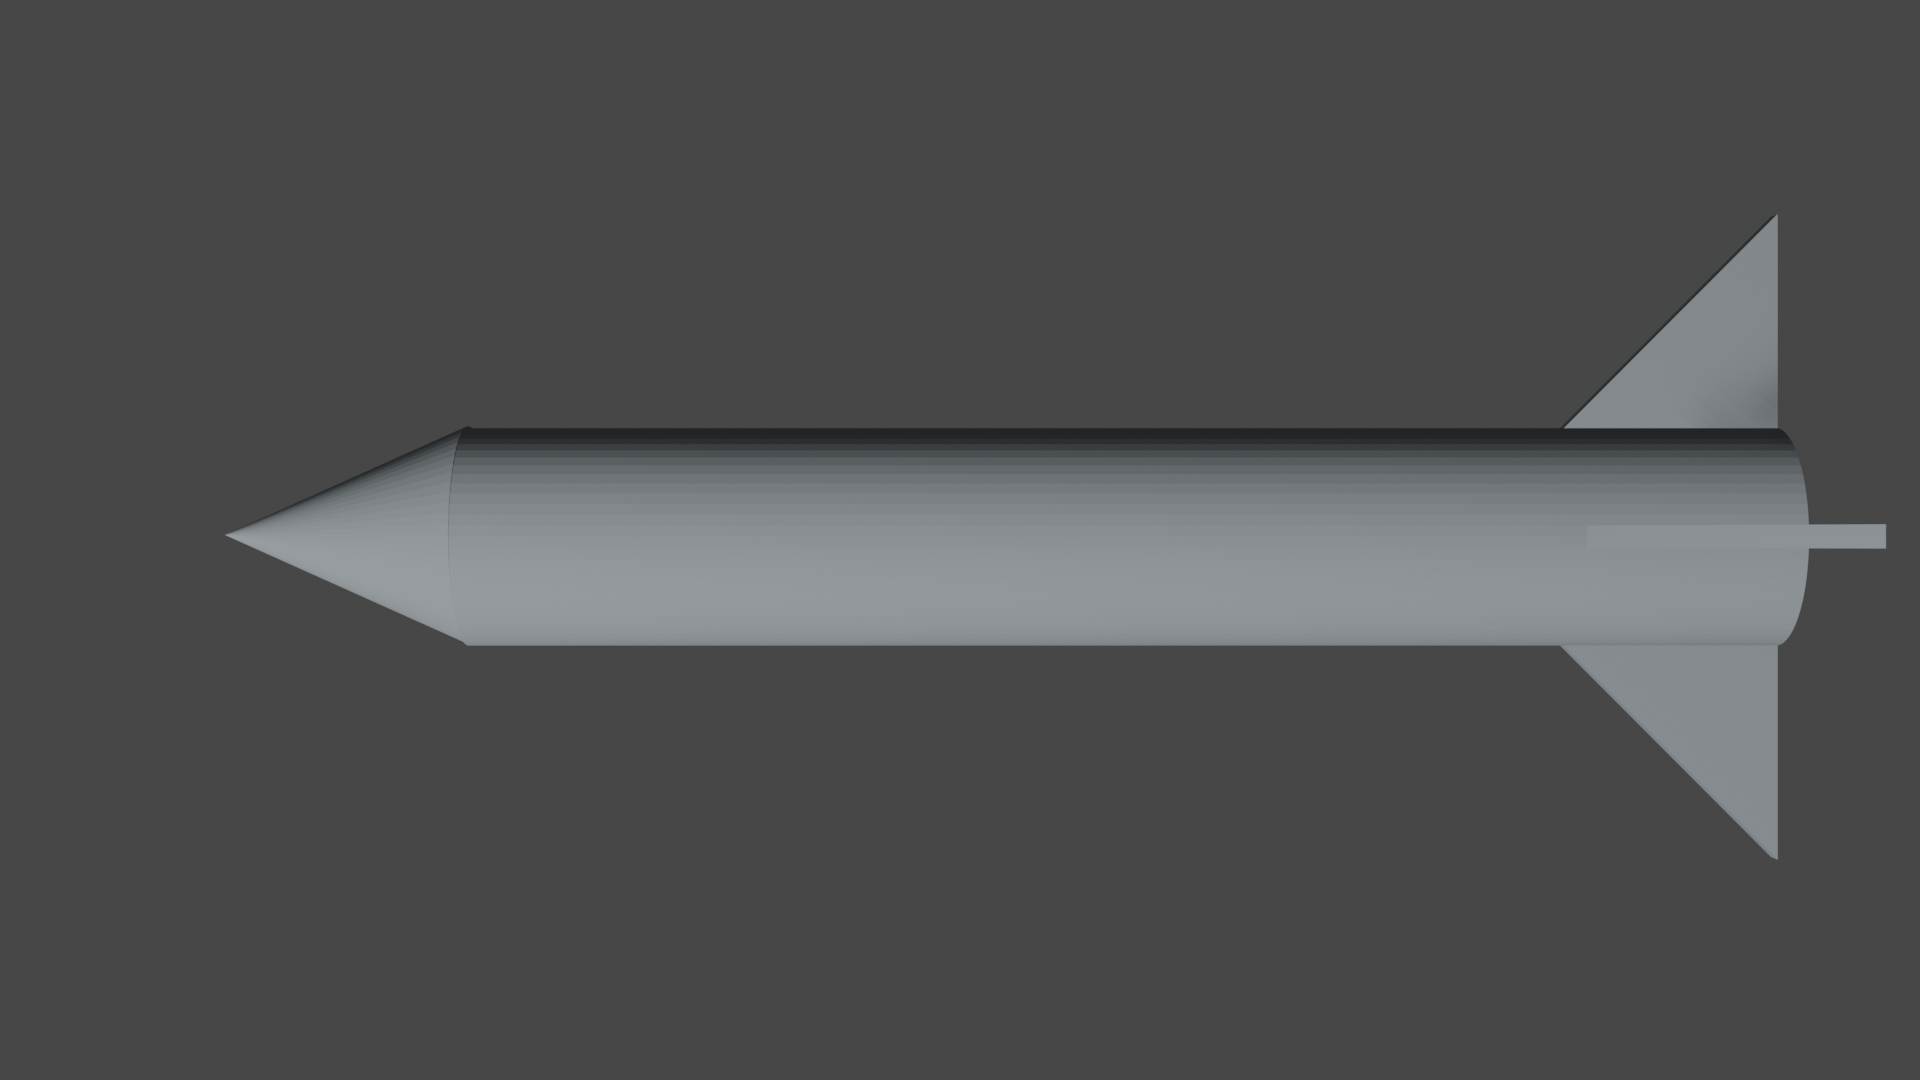
\includegraphics[width=.8\linewidth]{msl_top.png}
	  \end{subfigure}%
	  \begin{subfigure}{.5\textwidth}
	    \centering
	    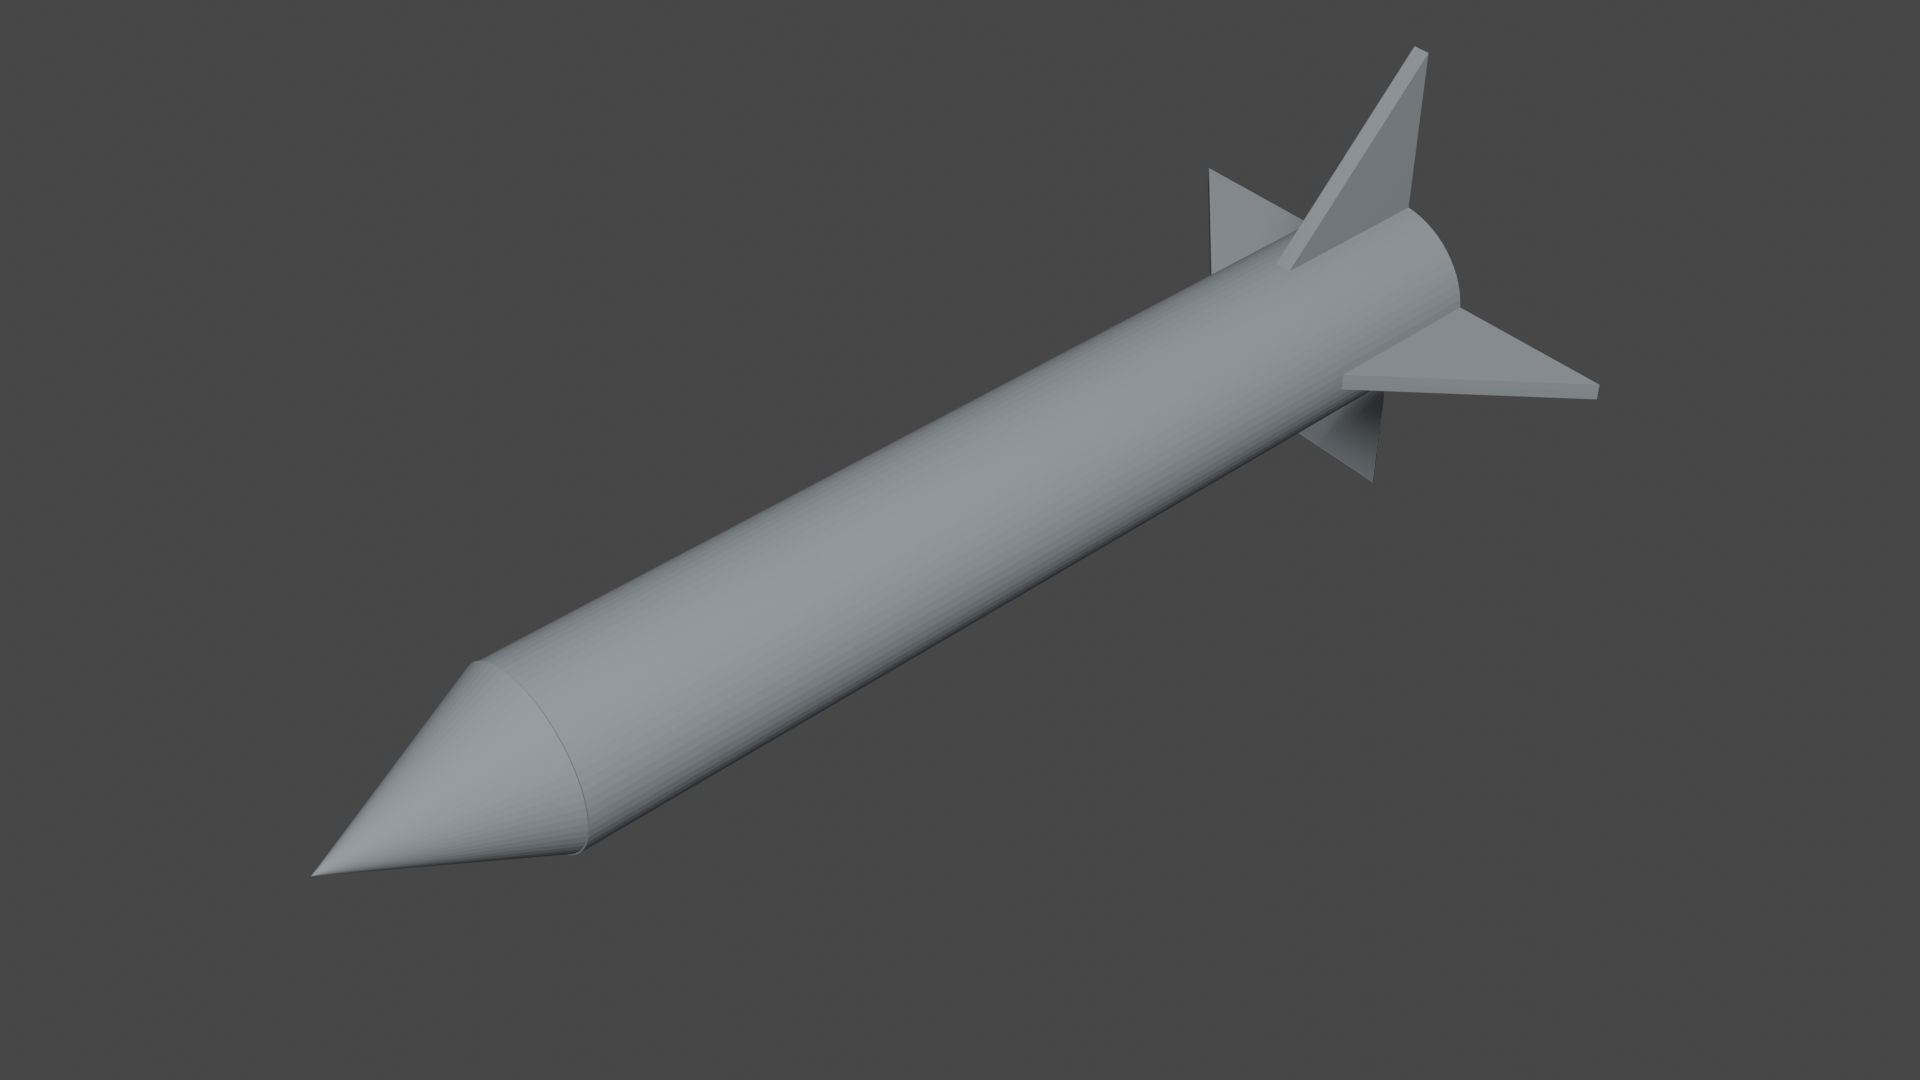
\includegraphics[width=.8\linewidth]{msl_side.png}
	  \end{subfigure}
	  \caption[Target missile]{Top and side view of a missile target.}
	  \label{fig:msl_target}
	\end{figure}

	\begin{figure}[htbp]
	  \centering
	  \begin{subfigure}{.5\textwidth}
	    \centering
	    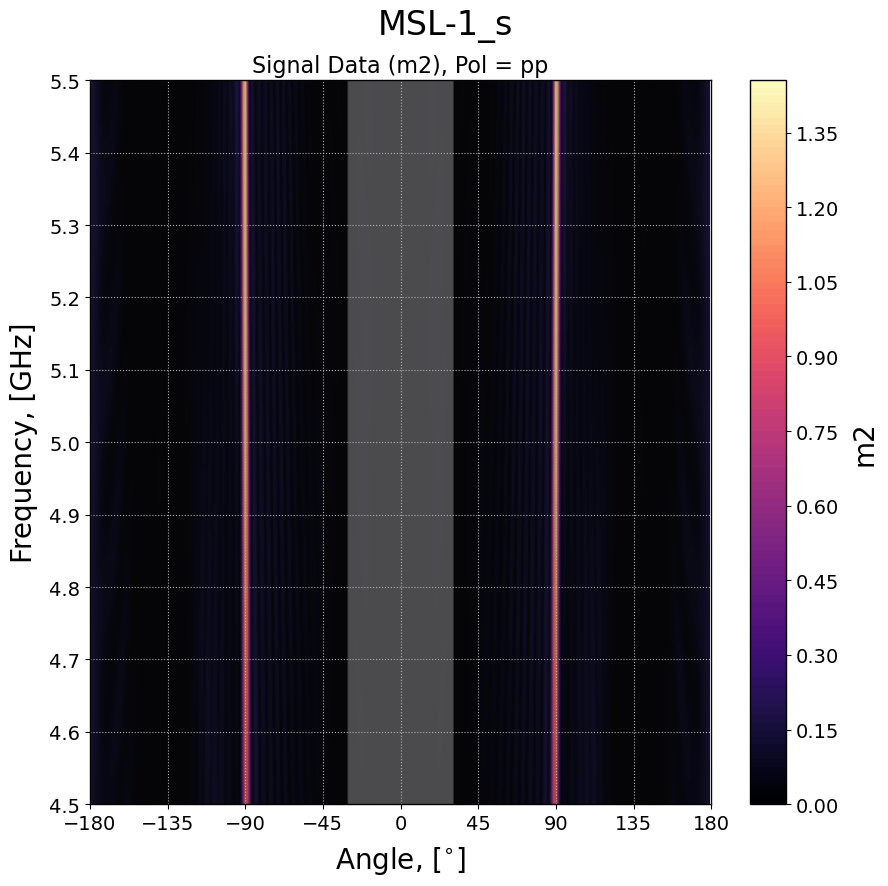
\includegraphics[width=.8\linewidth]{MSL-1_s_m2_pp.png}
	  \end{subfigure}%
	  \begin{subfigure}{.5\textwidth}
	    \centering
	    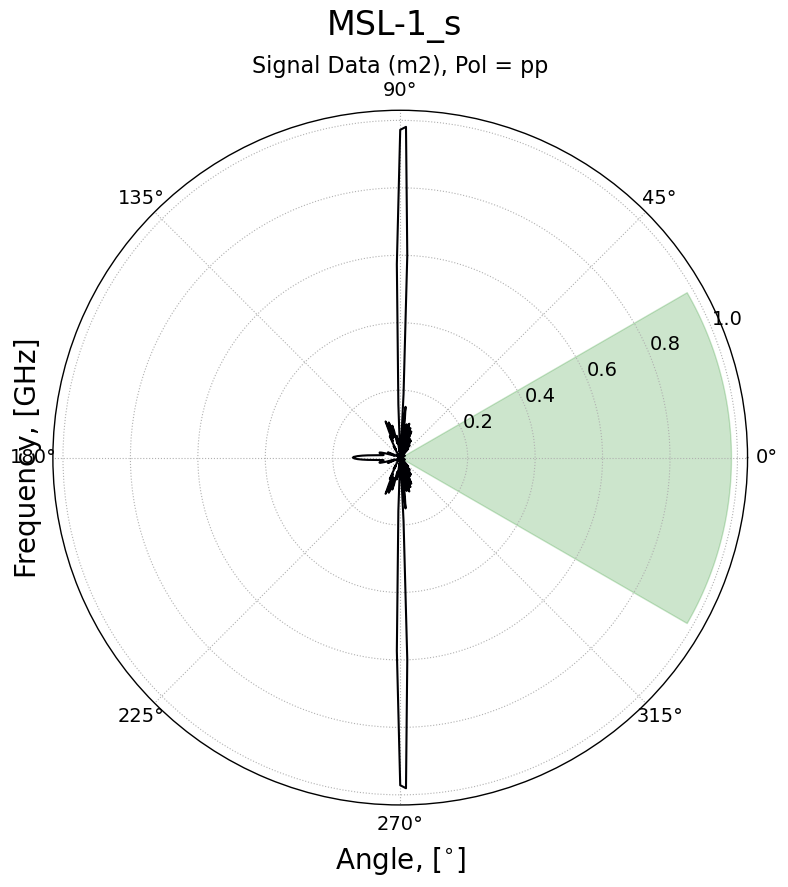
\includegraphics[width=.8\linewidth]{MSL-1_s_m2_pp_5GHz.png}
	  \end{subfigure}
	  \caption[Missile RCS data sample (Cut)]{An RCS measurement at 5 GHz over all angles, and the total RCS measurement of a missile target in $m^2$.}
	  \label{fig:msl_m2}
	\end{figure}

	\begin{figure}[htbp]
	  \centering
	  \begin{subfigure}{.5\textwidth}
	    \centering
	    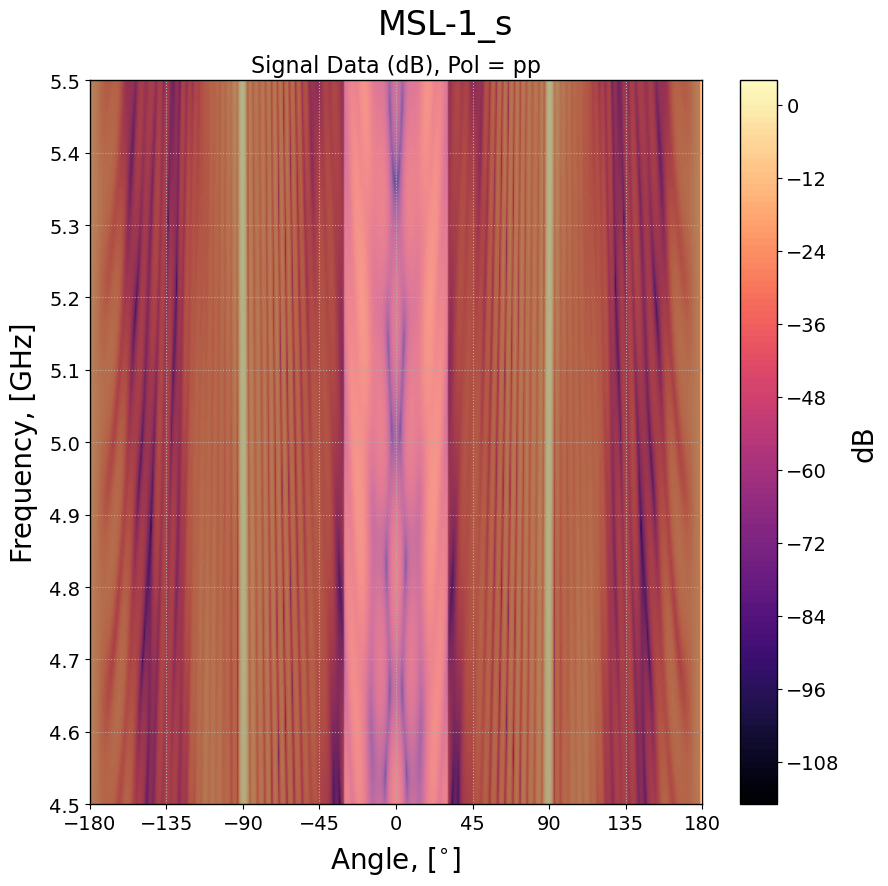
\includegraphics[width=.8\linewidth]{MSL-1_s_dB_pp.png}
	  \end{subfigure}%
	  \begin{subfigure}{.5\textwidth}
	    \centering
	    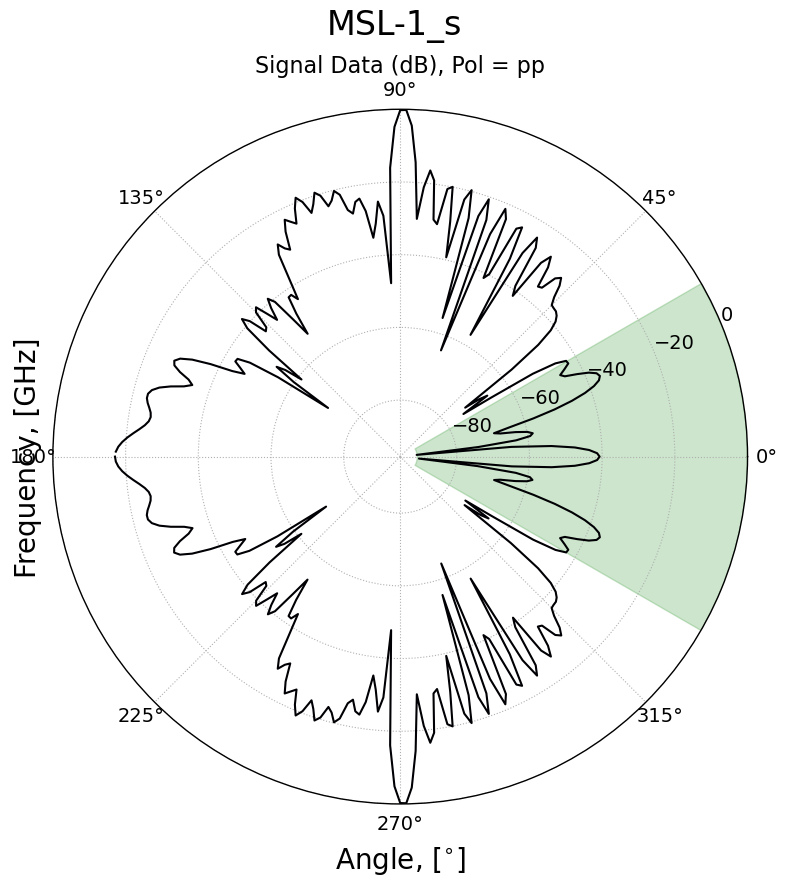
\includegraphics[width=.8\linewidth]{MSL-1_s_dB_pp_5GHz.png}
	  \end{subfigure}
	  \caption[Missile RCS data sample (Total)]{An RCS measurement at 5 GHz over all angles, and the total RCS measurement of a missile target in $\textrm{dB}_{sm}$.}
	  \label{fig:msl_db}
	\end{figure}

	The RCS cut of the model is used to give a quick at-a-glance view of the targets RCS deviation over angle. While this is useful on inspection, it is less useful for this project. Ideally, the sensor under examination would be able to make a classification using the data from a single angles measurement. This data would correspond to a single column of data taken from a total RCS contour plot. This single column contains 101 frequency measurements, ranging from 4.5 - 5.5 GHz. An example of frequency deviation for a single angle is shown in \ref{fig:freq_angle}. This project focuses heavily on this frequency deviation. Conceptually, the construction of each target should diverge enough to produce unique RCS responses.

	\begin{figure}[htbp]
	  \centering
	   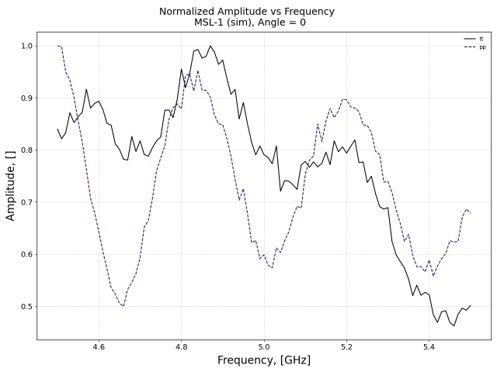
\includegraphics[width=.8\linewidth]{freq_angle.png}
	  \caption[Missile RCS data, Angle Slice]{Frequency deviation over a single angle.}
	  \label{fig:frq_ang}
	\end{figure}

\section{Machine Learning Models}

	Advance's in computer power, and the development of readily available software has made machine learning a common and powerful engineering tool. A machine learning model is an algorithm that is \textit{trained} rather than programmed. Training is the process of passing examples of a task or behavior to the model, and allowing it to adjust its \textit{parameters} to reach a desired outcome. The examples used to train a model include:  input data points or \textit{features}; and \textit{labels}, the expected outcomes for each set of features \cite{Chollet}.

	The application of machine learning models to radar signal classification has been thoroughly studied:  Deep Learning models, \gls{RNN}, tree regressors, random forests, state-vector machines as well as neural and \gls{CNN} have been documented to show promising performance \cite{ML_Radar_Survey}. The remote sensing community has also employed machine learning in target identification, which will be discussed in section \ref{sec:training}.

	Given the recent growth in CNN toolsets and previous success in classifying RCS frequency-series data this paper will focus on 1-Dimensional CNNs\cite{ML_RCS}. Originally developed to solve computer vision problems, CNNs are being employed with success in increasingly more problem sets to include radar signal classification, electro-cardiogram analysis, structural failure modes, and remote sensing \cite{CNN_Survey}. Two model topologies will be employed:  VGG-19, and ResNET. The first, VGG-19, is a simple, sequential, and very deep model. The second, ResNET, is a non-sequential residual network that favors `lateral' over vertical depth. Each topology will be discussed in detail in the following sections.

	\subsection{ Deep Learning}

		Convolutional Neural Networks are a subset of \textit{Deep Learning} models. `Deep' in this sense refers to depth-of-model as opposed to something philosophical \cite{Chollet}. The original deep learning networks were conceived in 1943 \cite{ANN} as artificial neural networks (ANNs). These networks borrowed from the construction of the human neuronal cortex to develop a simplified computation model based on a network of connected nodes. The nodes, or neurons of an artificial neural network are built to produce an output, for a given input. A perceptron, one of the simplest ANN architectures is shown in figure \ref{fig:percept} as an example \cite{Aurelien}.

		\begin{figure}[htbp]
		  \centering
		   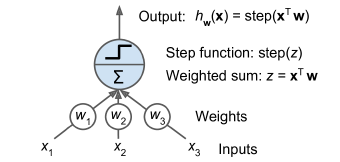
\includegraphics[width=.8\linewidth]{perceptron.png}
		  \caption[Perceptron node]{Perceptron model taken from `Hands on Machine Learning'\cite{Aurelien}.}
		  \label{fig:percept}
		\end{figure}

		The inputs $x_1, x_2, ... x_n$ are \textit{weighted} by $w_1, w_2, ...w_n$, summed using

		\begin{equation}
			z = w_1 x_1 + w_2 x_2 + ... w_n x_n = x^T w
		\end{equation}

		and passed to the perceptron. If the weighted sum $z$ is larger than some threshold, it will trigger the node's \textit{activation function}. An activation function is a response function that produces an output for a given input. Here, the activation function is a Heaviside step given as

		\begin{equation}\label{eq:heavy}
			h_w(x) = \textrm{step}(x^Tw).
		\end{equation}

		This activation function will step from zero to one if its threshold is reached. Alternate activation functions are detailed in the appendix. Deep learning models stack these weighted nodes into a `Dense' layer, and connected with other dense layers. The resulting series of connections and weights form the deep learning model's \textit{topology}.

		The weights for each node in the model are found using the following algorithm \cite{Chollet}:

		\begin{enumerate}
			\item Feed a batch of training samples to the model.
			\item Run the network for each sample $x$, and record the models prediction $y_{pred}$
			\item Compute the loss between samples label $y$ and $y_{pred}$
			\item Compute gradient of the loss with regard to the network's parameters
			\item Update the weights of the network in a way that slightly reduces the loss for the samples in the next batch
		\end{enumerate}

		Steps 1 and 2 take input data as a \textit{batch}, or a collection of multiple input samples has the model process them and make a prediction.  The `distance' between the sample's label $y$ and the model prediction $y_{pred}$ is measured using a \textit{loss function}. Steps 1 and 2 are called the \textit{forward pass}.	The process of updating the weights is done using \textit{stochastic gradient descent, (SGD)} and the \textit{back propogation} algorithm  \cite{BP}. When utilizing the TensorFlow package, all inputs, and model objects are tensors and can be manipulated using tensor operations. The SGD algorithm takes the tensor gradient of the model's loss function to determine a minima in step 4. Step 5 in the algorithm moves the weights away from this minima \cite{Chollet}.  Ideally, adjustments in the models parameters will reduce the loss function for the next batch of inputs.

		The concept of layers, weights, and the training algorithm are directly applicable to convolutional neural networks. The change from ANNs to CNNs is the structure of each `node' and the overall topology of the network.


	\subsection{Convolutional Neural Networks}

		Early neural networks were built using dense layers of nodes. The nodes of each layer connected to the nodes of other layers and interacted with varying levels of strength determined by their weights. These networks develop pattern recognition \textit{globally}. The entire input is considered when producing an output. Convolutional neural networks work to identify \textit{local} patterns \cite{Chollet}. This is done by using the process shown in figure \ref{fig:convo}.

		\begin{figure}[htbp]
			\centering
			 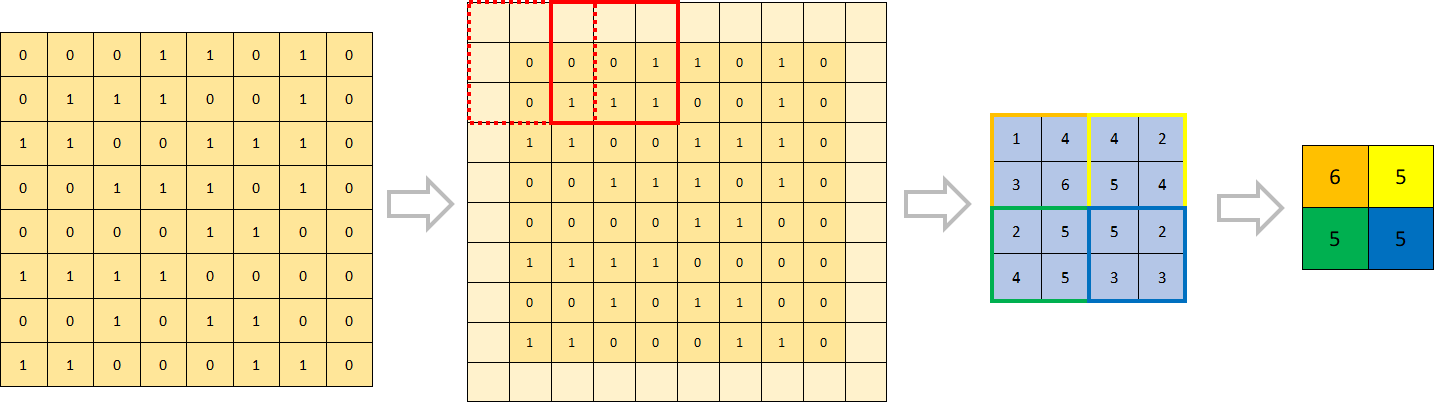
\includegraphics[width=\linewidth]{CNN_basics.png}
			\caption[CNN overview]{Convolution process:  Input Data -> Convolution -> Max Average.}
			\label{fig:convo}
		\end{figure}

		An 8x8 array of input data is passed to the model (orange). A padding (light orange) is applied to the perimeter, and the data is sampled by a convolution window (dotted red, 3x3). The convolution window performs a convolution operation on all data elements that fit inside it, before moving to the next batch of values (solid red, 3x3). The output of the convolution operation (which employs the layer's weights) is the \textit{kernal}, and is used to reassemble the data post convolution (light blue). The convolution window is then shifted by a distance determined by the layers \textit{stride}. In this case, the stride of the layer is 2. The convolution process is repeated until the entire input space has been sampled. The resulting output (blue) is then down-sampled using a pooling process. In this case, a pooling window of size 2x2, and stride 2 pulls the maximum value in its view. This is referred to as max pooling. Alternate pooling schemes such as average, and min pooling can also be employed.

		\subsubsection{VGG-19}

		Developed at the University of Oxford, the VGG topology was designed to increase accuracy for image recognition tasks. Utilizing a small receptive field, simple construction, and multiple stacks of convolution layers for each pooling operation, the VGG topology exceeded the performance of earlier CNN models \cite{VGG-19}. The key feature of the VGG topology is vertical depth. The developers found the increase in model depth was directly correlated with performance, particularly with complex inputs.

		This project utilizes the VGG-19 topology listed in table \ref{tab:vgg-19}. The convolution layers share a 1x3 receptive field, with a stride of 1 and `ReLu' activation functions. The max-pooling layers are 2x2 with a stride of 2. The convolutional layers terminate with a `flattening' layer. This layer prepares the convolutional data to be passed to a dense network. The a neural network features `dropout' layers. Drop out layers exclude samples within a batch, and help to prevent overfitting in the model. The final layer utilizes a `softmax' activation function. This activation calculates a probability for each label in the training data, and produces a prediction.

		\begin{table}
	    \centering
	    \begin{tabular}{|l|l|c|c|}
				\hline
		    Layer & Name & Input Shape & Output Shape  \\
				\hline
		    0 & Input & [101, 2] & [101, 2]\\
				1 & 1D-Conv(64) & [101,2] & [101, 64] \\
				2 & 1D-Conv(64) & [101,64] & [101, 64] \\
				3 & 1D-MaxPooling & [101,64] & [50, 64] \\
				\hline
				4 & 1D-Conv(128) & [50, 64] & [50, 128] \\
				5 & 1D-Conv(128) & [50, 128] & [50, 128]\\
				6 & 1D-MaxPooling & [50, 128] & [25, 128] \\
				\hline
				7 & 1D-Conv(256) & [25, 128] & [25, 256]\\
				8 & 1D-Conv(256) & [25, 256] & [25, 256]\\
				9 & 1D-Conv(256) & [25, 256] & [25, 256]\\
				10 & 1D-Conv(256) & [25, 256] & [25, 256]\\
				11 & 1D-MaxPooling & [25, 256] & [12, 256] \\
				\hline
				12 & 1D-Conv(512) & [12, 256] & [12, 512] \\
				13 & 1D-Conv(512) & [12, 512] & [12, 512] \\
				14 & 1D-Conv(512) & [12, 512] & [12, 512] \\
				15 & 1D-Conv(512) & [12, 512] & [12, 512] \\
				16 & 1D-MaxPooling & [12, 256] & [6, 256] \\
				\hline
				17 & 1D-Conv(512) & [6, 256] & [6, 512] \\
				18 & 1D-Conv(512) & [6, 512] & [6, 512] \\
				19 & 1D-Conv(512) & [6, 512] & [6, 512] \\
				20 & 1D-Conv(512) & [6, 512] & [6, 512] \\
				21 & 1D-MaxPooling & [6, 512] & [3, 512] \\
				\hline
				22 & 1D-Flatten & [3, 512] & [1, 1536] \\
				23 & Dense(4096) & [1, 1536] & [1, 4096] \\
				24 & Dropout(50\%) & [1, 4096] & [1, 4096] \\
				25 & Dense(4096) & [1, 4096] & [1, 4096] \\
				26 & Dropout(50\%) & [1, 4096] & [1, 4096] \\
				27 & Dense(1000) & [1, 4096] & [1, 1000] \\
				28 & Softmax(5) & [1, 1000] & [1, 5] \\
				\hline
			\end{tabular}
	    \caption[VGG topology]{Model dimensions}
	    \label{tab:vgg-19}
	  \end{table}


		\subsubsection{ResNET}

			\begin{description}
				\item [Batch Normalization: ]  Maintains a mean output close to zero, and the output standard deviation close to 1 \cite{Keras}.
				\item [Dropout: ] randomly sets input units to 0 with a frequency set by the \textit{dropout rate}. This helps to prevent overfitting during model training \cite{Keras}.
			\end{description}


\section{Optimizers and Augmentation}

Deep learning network optimizers utilize Neural network optimizers work best when the input data is augmented \cite{ML_RCS}. The augmentation processes used for this project are documented in section \ref{sec:DA}.

\section{Training}
\label{sec:training}

	Target recognition is the process of a sensor categorizing a target in its field of view given some training, or a pre-planned procedure. The remote sensing community has been experimenting with machine learning applications and their potential to increase classification accuracy for automatic target recognition with synthetic aperture radars. These ML models are pre-trained, and embedded within the radar receiver. A 2016 study documents three training regimes that have been employed to develop successful ML models:  1. Feature based training; 2. Semi-model based training; 3. Model based training \cite{SAR_Survey}.

	The similarity in operation of a SAR and traditional radar make these training regimes applicable to target identification in air defense radars. A strictly feature based approach would utilize an incomplete set of RCS measurements to train a sensor; a semi-model based approach would leverage the characteristics of a feature based test-set to create a more robust training set; and a model-based approach would attempt to create a full set of training data using model and simulation.

	This experiment will utilize a model-based training approach. The simulated RCS response of XX targets will be used to train a machine learning algorithm, and the accuracy of the model will be tested using measurement data.

	% Focus on feature based training
	\subsection{Feature-Based Training}
		The most common approach, feature based training utilizes either raw or template image-data to train a sensor. Template data is typically a snap-shot of a target in a specific `pose'. Pose in this context refers to the targets configuration with respect to the sensors viewing angle. Features include target size, configuration, as well as the statistical properties of the received signal.  While deeply researched and computationally accessible, feature based training suffers from statistical classification breakdown and pattern recognition problems \cite{SAR_Survey}. Governments and their militaries go to great lengths to set a standard for how national secrets are classified and controlled \cite{EO_10290}\cite{PLA_Class}, restricting the amount of reliable template data available for training.

		Borrowing this concept for training a traditional radar:  assume a template image to be the echo response from a target at a single aspect-angle. This template will contain useful features for training a machine learning model. However, if the amount of templates for a target are limited, the model could over-train to the incomplete information and miss-classify unfamiliar pose angles.

	\subsection{Semi-Model Based Training}
		Semi-model based training extends the concept of feature based training, while attempting to build a more complete training set given limited template data.

		Semi-model training data seeks to extract characteristic data from the training templates:  scattering center locations, counts, and intensities are used to generalize the expected response from the target. from both feature and model based training: the limited feature based data set is processed to produce scattering center models. This method seeks the best of both world:  robust, `behavior' based models that are built with limited, but readily available data sets.

	\subsection{Model-Based Training}
		Model based training utilizes ESIM software to produce training data. In its simplest conception, the `model based' approach can be thought of as a data generator for a feature based training regime. That is, a system can be trained to identify features using modeled data, providing a sensor with otherwise inaccessible data.

		Alternately, generated models can be processed to provide the sensor with a more `bottom-up' training approach. The `bottom-up' concept was developed and implemented by Robert A. Brooks at MIT for the ACRONYMN target recognition system \cite{Brooks}\cite{Brooks2}. This method shifts the focus of training away from what the target looks like in a specific, limited instance and focuses on the more general representation of \textit{how} the target \textit{may} look.

\phantomsection
\chapter{Methodology}
\label{ch:methodology}
\glsresetall


\section{Targets}

  Five target models were chosen for this experiment. Each model is a missile-surrogate with a shared fuselage, and a unique nose cone. The dimensions of the fuselage and the nose cones are listed in table \ref{tab:models}. Nose cones 1-3 are simple cones with a fixed base diameter and edge length. Nose cones 4 and 5 are curved. They share the common 3 inch base diameter, with  differing diameters as they extend from the base to tip. The additional measurements represent the diameter of the cone at equally spaced intervals along the edge from base to tip. Each model is made of aluminum as is assumed to behave as a PEC in the presence of EMR. The Cad models of each missile nose is shown in figures \ref{nose_1_2}, \ref{nose_3_4}, and \ref{nose_5}. The side and top view of the missile is shown in figure \ref{fig:missile_body}.

  \begin{figure}[htbp]
    \centering
    \begin{subfigure}{.5\textwidth}
      \centering
      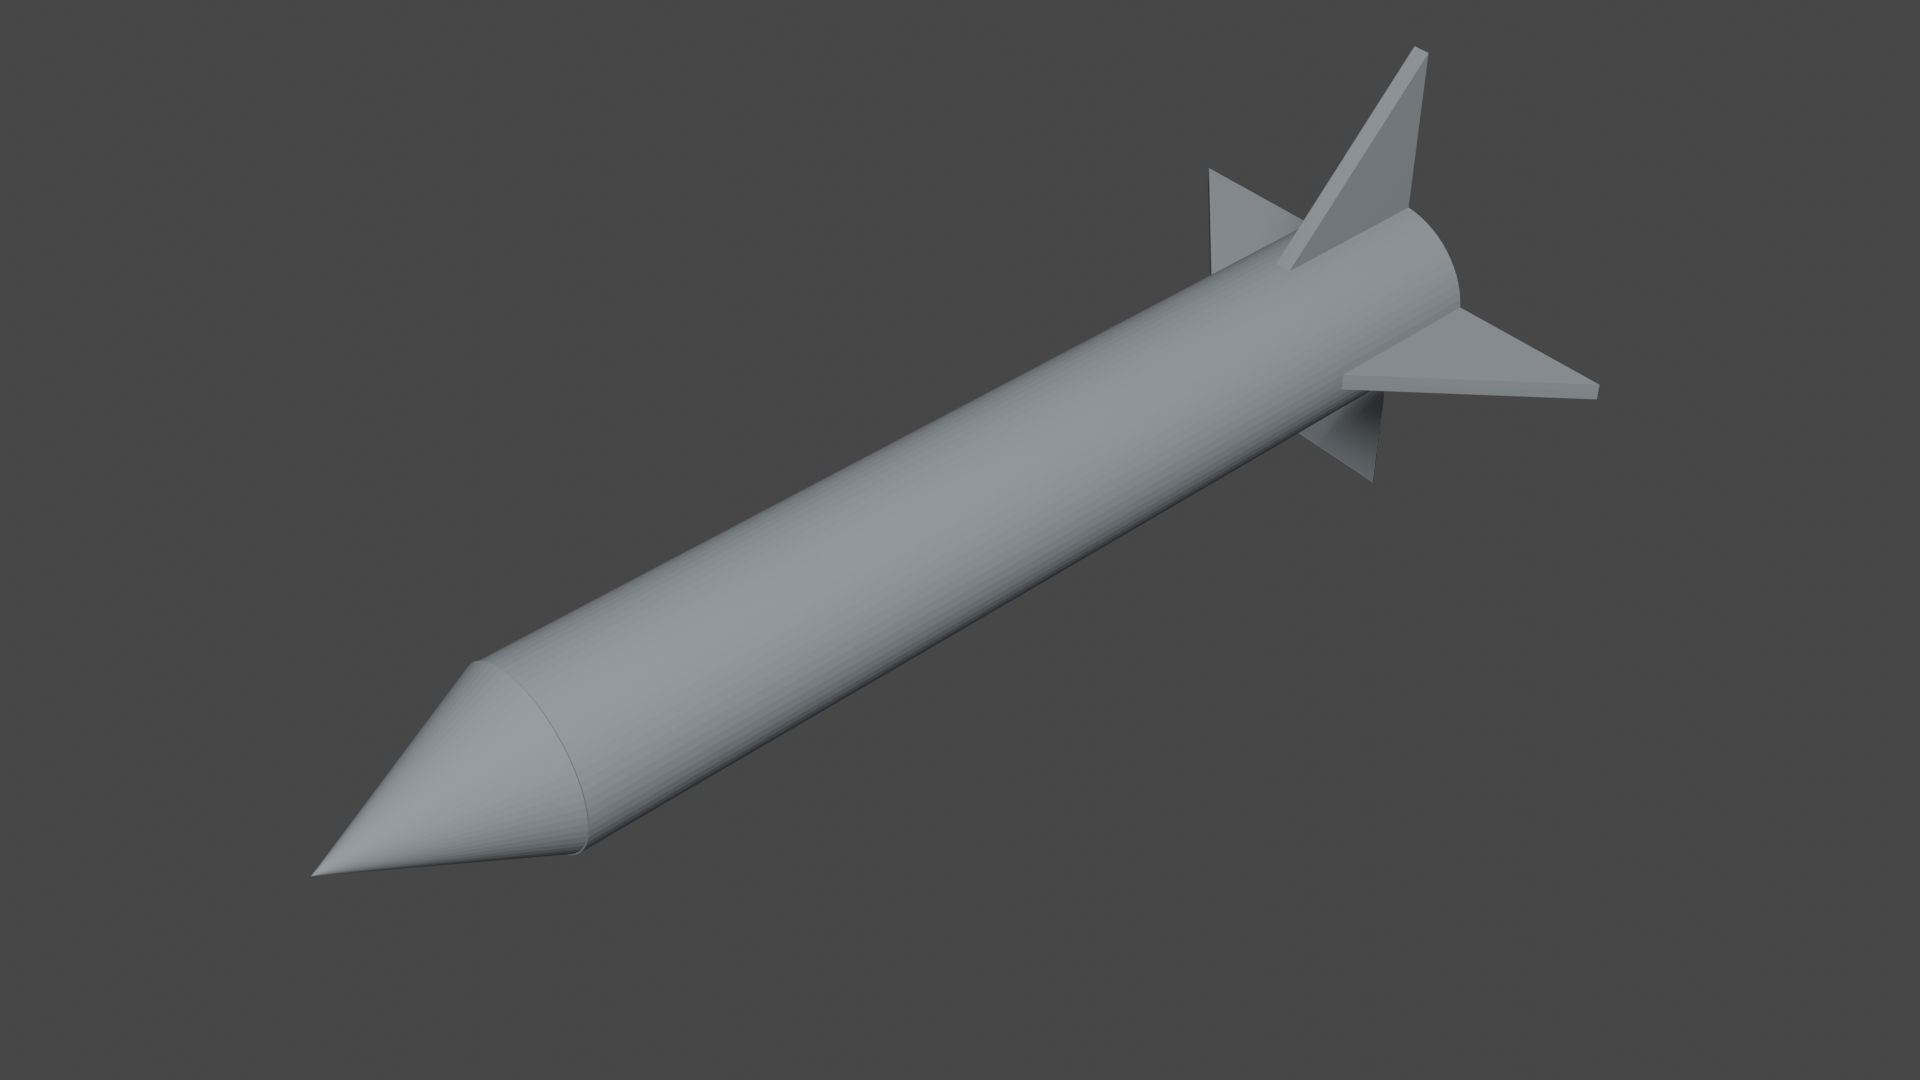
\includegraphics[width=.8\linewidth]{msl_side.png}
    \end{subfigure}%
    \begin{subfigure}{.5\textwidth}
      \centering
      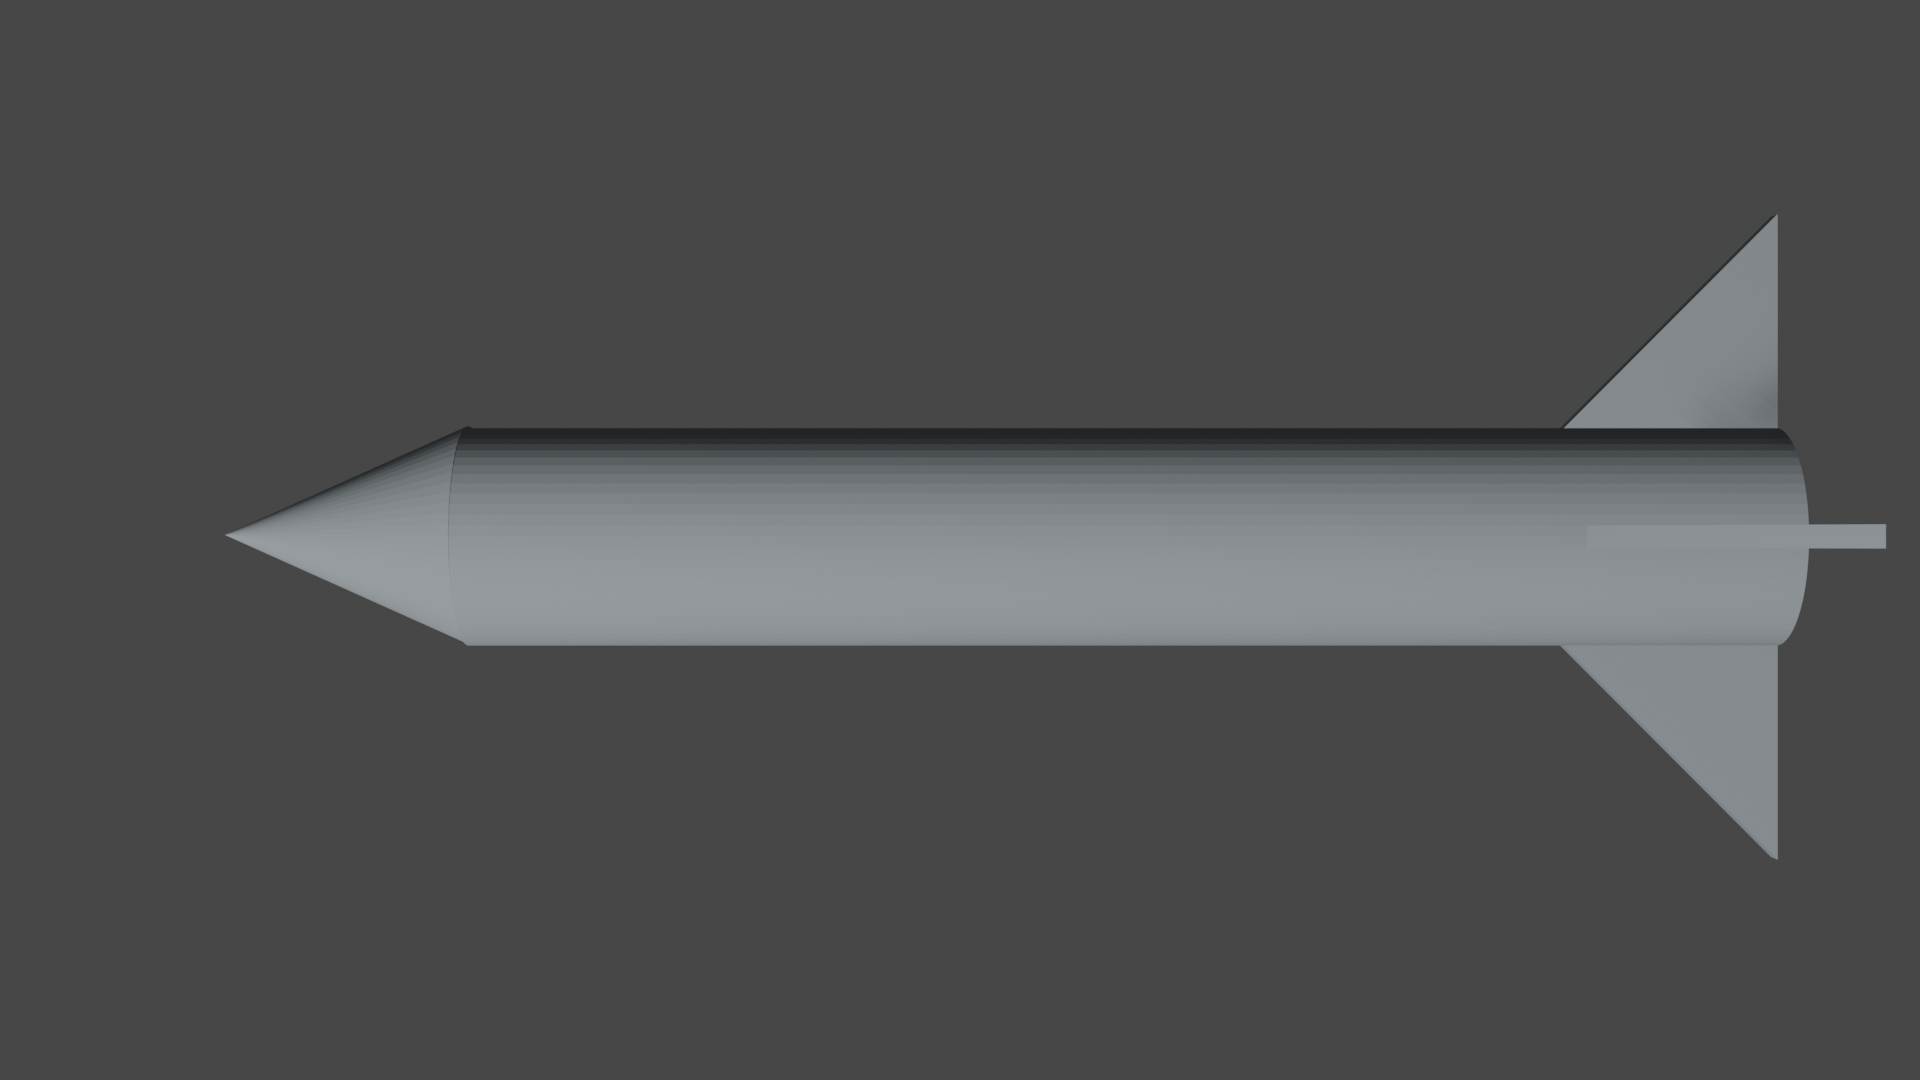
\includegraphics[width=.8\linewidth]{msl_top.png}
    \end{subfigure}
    \caption{Side and top view of the missile surrogate (Cad model)}
    \label{fig:missile_body}
  \end{figure}

  Simulation models were developed using Blender 3d, and exported as .stl mesh models. Mesh models were converted to solids form mesh, and exported as .step geometries using FreeCad. The .step format worked well with CADFeko's internal meshing system. Since Blender 3D does not export .step natively, the additional step of importing the .stl mesh into FreeCad was necessary.

\section{Measurement}
  The targets were measured at the Air Force Institute of Technologies (AFIT) Compact Radar Range. The layout of the AFIT range is shown in figure \ref{fig:range}. The range uses a BlueMax G6 instrumentation radar (blue items in schematic), with a Vivaldi wide-band antenna configured in both horizontal and vertical polarizations. Transmitted signals are directed at a curved reflector located 3 meters from the antenna. Ideally, the incident field will be a plane wave. That is, the wave front is the same when measured vertically or horizontally. However, the short distance between the antenna and the target will produce a curved wave-front surface. The reflector helps to `flatten' the wave front, and make it appear more planer.

  Targets are placed on a foam column located 7 meters from the reflector. The column is 2 meters tall, and can rotate 360 degrees. Foam is used, as its intrinsic properties are similar to air, and do not contribute significantly to scene clutter.

  \begin{figure}[htbp]
    \centering
    \begin{subfigure}{.8\textwidth}
      \centering
      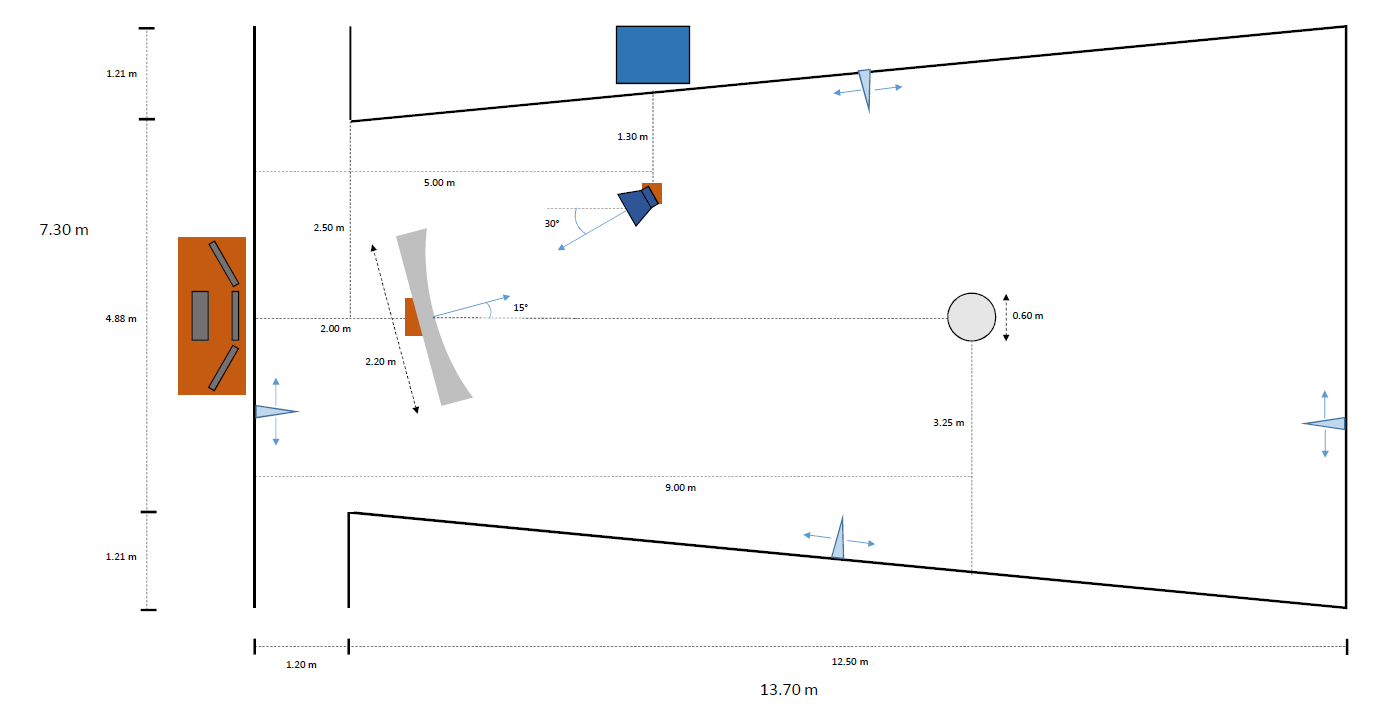
\includegraphics[width=.8\linewidth]{range.png}
    \end{subfigure}%
    \begin{subfigure}{.8\textwidth}
      \centering
      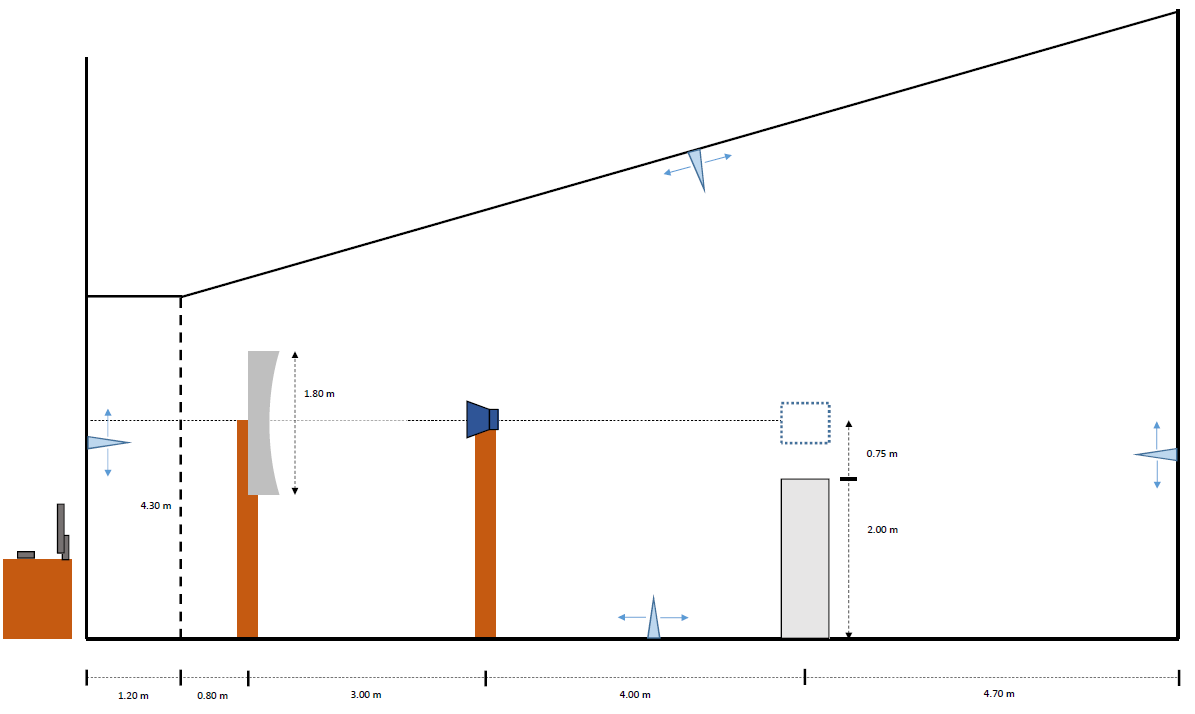
\includegraphics[width=.8\linewidth]{range_side.png}
    \end{subfigure}
    \caption[AFIT Compact Range Schematic]{Top-down and side view of the AFIT compact radar range.}
    \label{fig:range}
  \end{figure}

  The radar can capture measurements over multiple frequencies, polarizations, and target aspect-angles. Measurements are returned as complex voltages $M$. A measurement is collected using a specific carrier frequency $f$, at a single aspect angle $a$. For example, measurement $M_0$ is collected by launching a stream of pulses with carrier frequency $f_0$ at a target presenting a fixed aspect angle $a_0$. The receiver will collect and integrate $N$ echo pulses and store the value as $M(f_0, a_0)$. This process is repeated over the desired range of frequencies and angles resulting in a matrix

  \begin{equation}\label{eq:RCS_mat}
    E_{tt} =
     \begin{bmatrix}
       M_{0,0} & M_{0,1} & \cdots & M_{0,A} \\
       M_{1,0} & M_{1,1} & \cdots & M_{1,A} \\
       \vdots  & \vdots  & \ddots & \vdots  \\
       M_{F,0} & M_{F,1} & \cdots & M_{F,A}
     \end{bmatrix}
     \\
     E_{pp} =
      \begin{bmatrix}
      M_{0,0} & M_{0,1} & \cdots & M_{0,A} \\
      M_{1,0} & M_{1,1} & \cdots & M_{1,A} \\
      \vdots  & \vdots  & \ddots & \vdots  \\
      M_{F,0} & M_{F,1} & \cdots & M_{F,A}
      \end{bmatrix}
  \end{equation}

  where $E_{tt}$ and $E_{pp}$ represent measurements taken for the vertical and horizontally aligned incident wave polarization. Each row in the matrices corresponds to 360 aspect angles measured at one frequency. The total array shape is $F \times A$, where $F$ and $A$ are the number of frequencies and angles captured respectively.

  Table \ref{tab:m_params} lists the measurement parameters used for this experiment.

  \begin{table}
    \centering
    \begin{tabular}{|l|r|}
      \hline
      Transmitter Power: & $40$[dBm]\\
      \hline
      Tx Gain: $15$[dB]\\
      \hline
      Rx Gain: $15$[dB]\\
      \hline
      IF BW: $200$[kHz]\\
      \hline
      Noise Figure, $F$:  $3$[dB]\\
      \hline
      Tx Loss: $4.5$[dB]\\
      \hline
      Rx Loss: $4.5$[dB]\\
      \hline
      Operating Temp: $68$[F]\\
      \hline
      Pulse Width: & $10[ns]$\\
      \hline
      Frequency Range: & $4.5-5.5 [GHz]$, $10 [MHz]$ step\\
      \hline
      Aspect-angle Range: & $0-360 ^{\circ}$, $1^{\circ}$ step\\
      \hline
      Integration Factor: & $1024$ \\
      \hline
      Transmit Delay : & $330$ [ns] \\
      \hline
      Receiver Delay : & $434-446$ [ns] \\
      \hline
    \end{tabular}
    \caption{Measurement parameters.}
    \label{tab:m_params}
  \end{table}

  % TODO: add quiet zone information

  The radar used for this project produces a discrete RCS measurement at individual frequencies as opposed to a time domain response for each pulse. Since this time-domain information was unavailable, this experiment attempts to recreate the time-domain response, by capturing discrete measurements for each frequency and stitching them together into a frequency domain equivalent for the expected time-domain response.

  The integration factor was chosen to provide sufficiently accurate measurements. This ideal measurement serves as a signal to noise performance baseline. The receiver delay of $434-446$ [ns] puts the quiet zone window at approximately 76 meters when accounting for the reducing transmission speed of waves in transmission line. The target fixture is located 14 meters from the antenna, with the remaining distance accounted for by feedline from the instrument to the antenna. This window was confirmed by `walking` the range. This operation transmits pulses from the antenna, and shifts the reception window until a known target is captured in the desired quiet zone.

\section{Simulation}

  Simulations were completed using Altair's CADFeko Electromagnetic Simulation Suite. CADFeko uses an iterative \gls{MOM-SEP} algorithm to compute the RCS response of the target model. The output data from the simulation is in phasor form. Method of Moments is used to calculate scattering for targets in the resonant regime:  when physical target size is roughly the same size as the incident wave length, but less than 10 times larger \cite{Knott}. At 5 GHz, the incident wave length is 60 millimeters. At 457mm, the fuselage body is 7.62 times larger than the 5 GHz wavelength placing towards the upper end of the resonant regime. The nose cones range in size from 101 to 228 mm, which fit comfortably in the resonant regime.

\section{Data Processing}

  \subsection{Data Set Generation}
    In order to mimic the expected response of a radar pulse, training and test data sets are built by slicing the RCS matrices shown in equation \ref{eq:RCS_mat} column wise. The resulting vectors

    \begin{equation}\label{eq:F_vec}
      F_{tt}(f, a_n) =
       \begin{bmatrix}
         M_{0, a_n} & M_{1,a_n} & \cdots & M_{F,a_n}
       \end{bmatrix},\,\,
       \\
     F_{pp}(f, a_n) =
      \begin{bmatrix}
        M_{0, a_n} & M_{1,a_n} & \cdots & M_{F,a_n}
      \end{bmatrix}
      \\
    \end{equation}

    contain the measurements $M(f, a_n)$ for all frequencies $f$, at a specified angle $a_n$ for the vertical and horizontal polarizations respectively. Each vector corresponds to the frequency content of an integrated pulse stream for each pose angle of the target. The training data set can be made arbitrarily large by multiplying frequency slices and applying random additive noise with power $N_{train}$ to create variance in each sample.

    Each sample in the training data set is assigned a label that corresponds to the `sector' that each sample falls in. Sectors are chosen such that RCS characteristics specific to the target fall in the same sector. This experiment utilizes either 3 or 4 90-degree sectors centered on the nose, tail, and sides of the target. The three label case collapses the sides of the fuselage into a single label.

    Test data sets are built similarly:  frequency vectors  are extracted from the measurement array, and additive noise with power level $N_{test}$ is applied.

  \subsection{Data Augmentation}
  \label{sec:DA}

    During training, neural networks optimize their decision weights by utilizing an `optimizer'. An optimizer is a method of testing whether the network is adjusting it weights in a way that maximizes its ability to categorize the input data correctly. This experiment utilizes a Stochastic Gradient Descent optimizer (SGD). This method favors adjustments in the networks weights that push towards a minimization of error in categorization. Since this is a method that utilizes slopes, differentiation is employed. In order to prevent unnecessarily large slopes, data is augmented. There are two forms of data augmentation that are typically employed: standardization, and normalization.

    Standardization takes the maximum value in the current training array, and scales the entire array. This creates a data range between 0 and 1. Standardization of data in this experiment is done using

    \begin{equation}\label{eq:F_stan}
      F_{tt}(f, a_n) =
       \begin{bmatrix}
         M_{0, a_n} & M_{1,a_n} & \cdots & M_{F,a_n}
       \end{bmatrix} / max(F_{tt}(f, a_n))
    \end{equation}

    where the function $max()$ pulls the max value in the vector.

    Normalization extracts the mean and standard deviation of the vector and returns a `Z-Score' for the each cell in the array using

    \begin{equation}\label{eq:F_z}
      F_{tt}(f, a_n) =
       \frac{\left(
       \begin{bmatrix}
         M_{0, a_n} & M_{1,a_n} & \cdots & M_{F,a_n}
       \end{bmatrix}
        - \mu \right)}{\sigma}
    \end{equation}

    where $\mu$ is the mean value of the vector, and $\sigma$ is the standard deviation.

  \subsection{Comparison}
  \label{sec:comparison}

    Signals are compared using a cross-correlation function. The cross correlation function measures the similarity between two signals, and outputs a correlation coefficient, $\rho$. Values for $\rho$ range from $\pm 1$ for correlated, and anti-correlated signals respectively, and $0$ for un-correlated signals. As an example, the cross correlation of a signal with itself, will have $\rho=1$.

    Signal similarity is measured over all frequencies, at each angle using

    \begin{equation}\label{eq:corr}
      \rho = Corr( E_{1, tt/pp}(f, a_i), E_{2, tt/pp}(f, a_i)  )
    \end{equation}

    where $E_{1, pol}$ and $E_{2, pol}$ RCS phasor response measurements for signals 1 and 2, at angle $a_i$ and polarization $pol$, over all frequencies $f$. Signals will be selected from the pool of simulated and measured RCS response. Measuring the correlation strength of all targets with one another will serve as a means of identifying breakdowns in target classification. The correlation function is always applied to signals with similar polarizations.

    To measure the breakdown in signal correlation as noise is applied, the following algorithm is employed:

    \begin{enumerate}
      \item Signals 1 and 2 are selected
      \item Noise is applied to signal 1 and signal 2
      \item Signals one and two are augmented per angle
      \item Equation \ref{eq:corr} is applied for each angle
      \item The resulting vector of correlation coefficients is plotted against angle
    \end{enumerate}

    Correlation performance is reported in SNR. The SNR for each target is the average phasor value of all data elements in the matrices $E_{tt}$ and $E_{pp}$ for each target.


\section{Neural Network Development}




\section{RCS Calculation}

\phantomsection
\chapter{Results and Analysis}
\label{ch:results}
\glsresetall
\section{Preamble}

Preamble text here.

\section{Section Title}
\label{sec:sectionTwoRef}

Reference equations a little differently like \labelcref{eq:eqRefNameHere}. Or reference a table like \Cref{tab:tabRefNameHere}.

\begin{table}[tb!]
	\begin{center}
		\caption[TOC Table Title Here]{Table Title Here}
		\label{tab:tabRefNameHere}
		\begin{tabular}{l|S|r} % <-- Changed to S here.
			\textbf{Description} & \textbf{Variable} & \textbf{Value} \\
			\hline
			Focal lengths & $f_x$ & \num{198.44397844114553} \\
			%			Focal length, y   
			& $f_y$ & \num{198.82574577980597} \\
			\hline
			Image Center & $c_x$ & \num{104.82882039668912} \\
			%			Image Center, y  
			& $c_y$ & \num{92.83779928839462} \\
			\hline
			Radial Distortion& {$k_1$} & \num{-0.39351276662408013} \\
			%			Radial Distortion 
			& {$k_2$} &  \num{0.1559033641626471} \\ 
			%			Radial Distortion 3
			& {$k_3$} & 0  \\
			\hline	
			Tangential Distortion & {$p_1$} & \num{-0.12466011637578988e-3} 
			\\
			%			Tangential Distortion 2
			& {$p_2$} &  \num{-1.6292737247630268e-3} \\ 
		\end{tabular}
	\end{center}
\end{table}
\phantomsection
\chapter{Conclusions}
\label{ch:conclusion}
\glsresetall
{
Conclusion text here.
}
\section{Future Work}
{
Text here

\begin{itemize} % bulleted list
	
	\item Item 1 text here.
	
	\item Item 2 text here.

\end{itemize}
}
\phantomsection
%%%%%%%%%%
% if Appendix is needed:
%%%%%%%%%%
\renewcommand{\theHchapter}{A\arabic{chapter}}
\appendix
%	\begin{appendices}
\phantomsection

\chapter{Model Measurements}
\label{app:model_measurements}
  \begin{table}
    \centering
    \begin{tabular}{lrl}
    Name & Dimension & Unit [in] \\
    fuselage & Length & $18$\\
            & Diameter &  $3$\\
            & Fin     & $2 \frac{5}{16}$\\
            \\
    Nose-1  & Base & $3$ \\
            & Edge Length & $3 \frac{11}{16}$ \\
            \\
    Nose-2  & Base & $3$ \\
            & Edge Length & $5 \frac{13}{16}$ \\
            \\
    Nose-3  & Base & $3$ \\
            & Edge Length & $8 \frac{11}{16}$ \\
            \\
    Nose-4  & Base & $3$ \\
            & Diameter 1 & $2.91339$ \\
            & Diameter 2 & $2.56$ \\
            & Diameter 3 & $1.57$ \\
            \\
    Nose-5  & Base & $3$ \\
            & Diameter 1 & $2.87$ \\
            & Diameter 2 & $2.52$ \\
            & Diameter 3 & $1.89$ \\
            & Diameter 3 & $0.83$ \\
    \end{tabular}
    \caption{Model dimensions}
    \label{tab:models}
  \end{table}

\chapter{Models}
\label{app:models}

  \begin{figure}[htbp]
    \centering
    \begin{subfigure}{.5\textwidth}
      \centering
      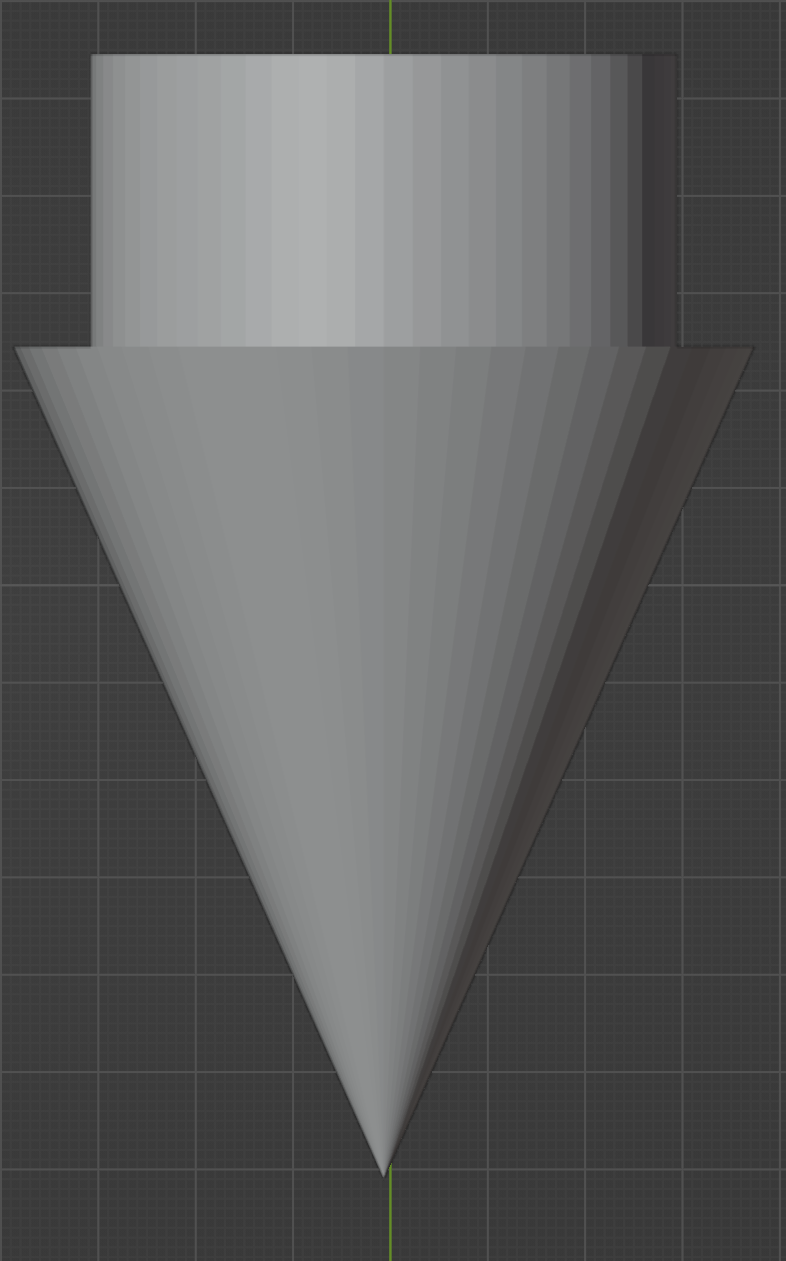
\includegraphics[width=.8\linewidth]{nose_1.png}
    \end{subfigure}%
    \begin{subfigure}{.5\textwidth}
      \centering
      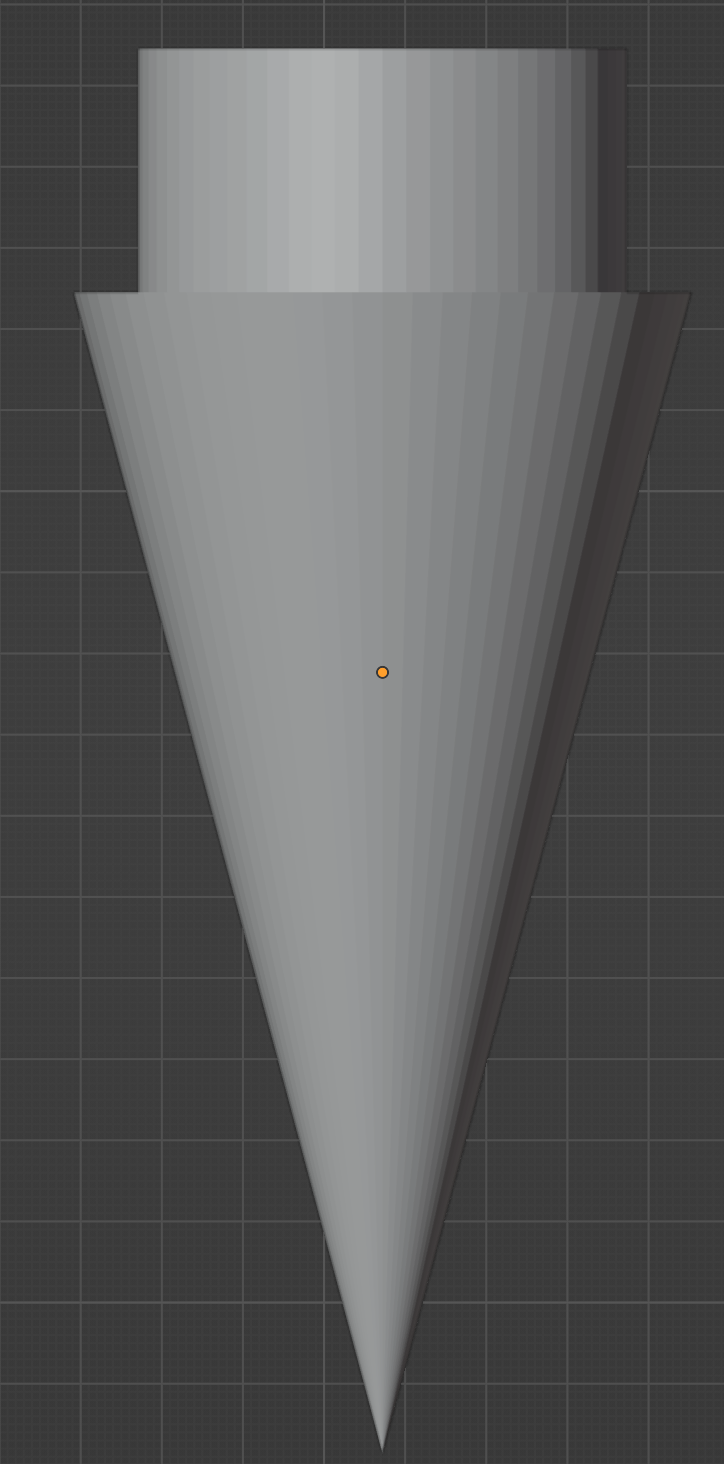
\includegraphics[width=.8\linewidth]{nose_2.png}
    \end{subfigure}
    \caption{Simulation targets 1 and 2}
    \label{fig:nose_1_2}
  \end{figure}

  \begin{figure}[htbp]
    \centering
    \begin{subfigure}{.5\textwidth}
      \centering
      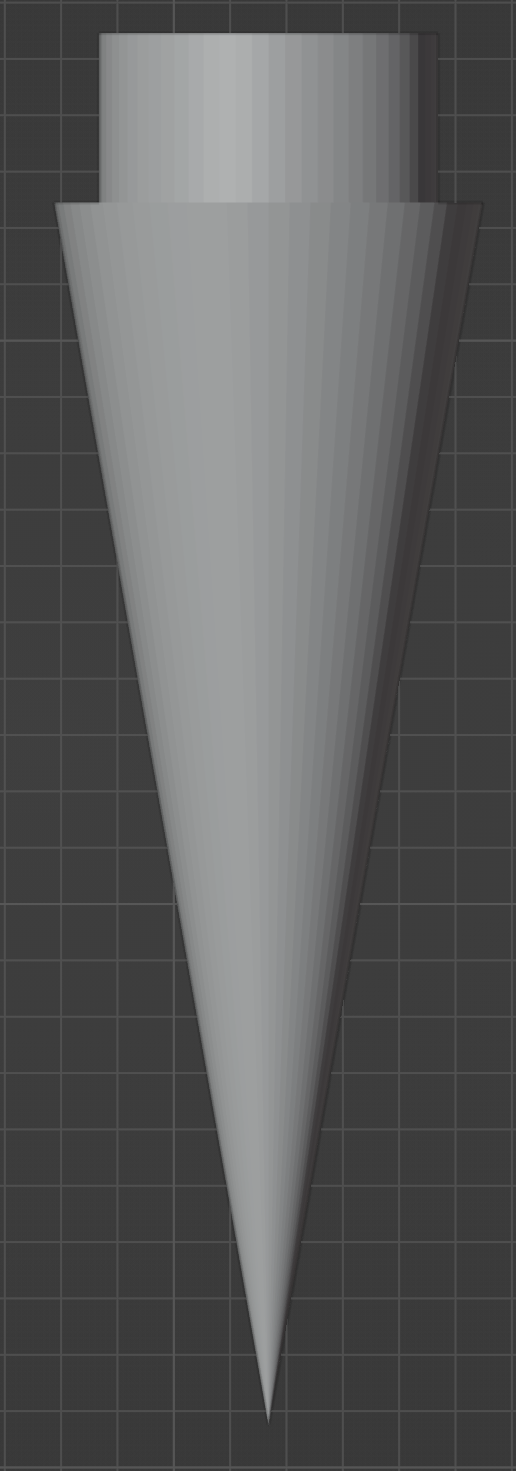
\includegraphics[width=.8\linewidth]{nose_3.png}
    \end{subfigure}%
    \begin{subfigure}{.5\textwidth}
      \centering
      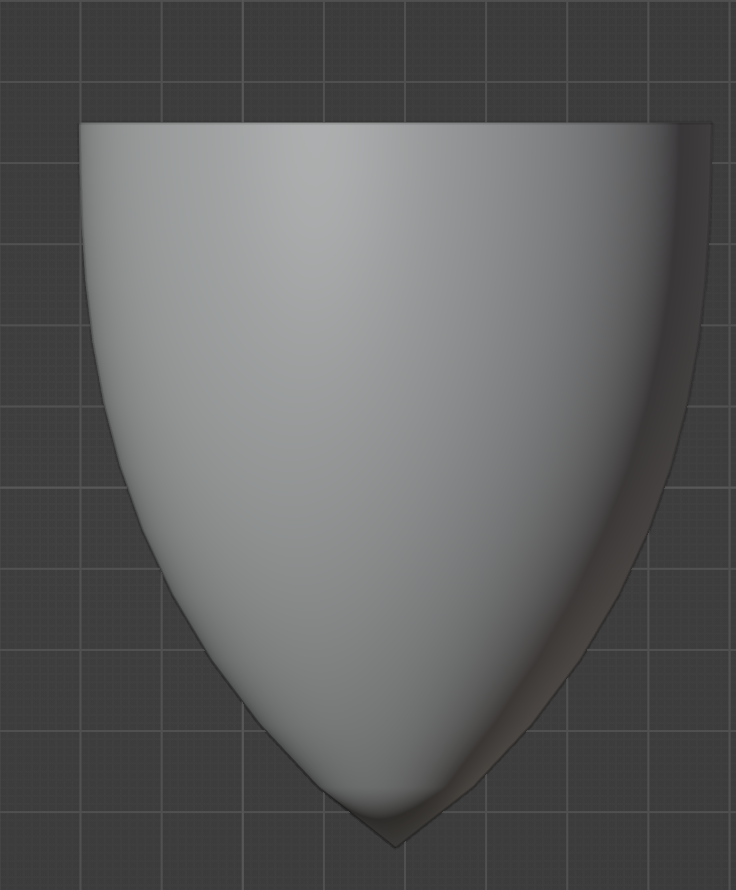
\includegraphics[width=.8\linewidth]{nose_4.png}
    \end{subfigure}
    \caption{Simulation targets 3 and 4}
    \label{fig:nose_3_4}
  \end{figure}

  \begin{figure}[htbp]
    \centering
    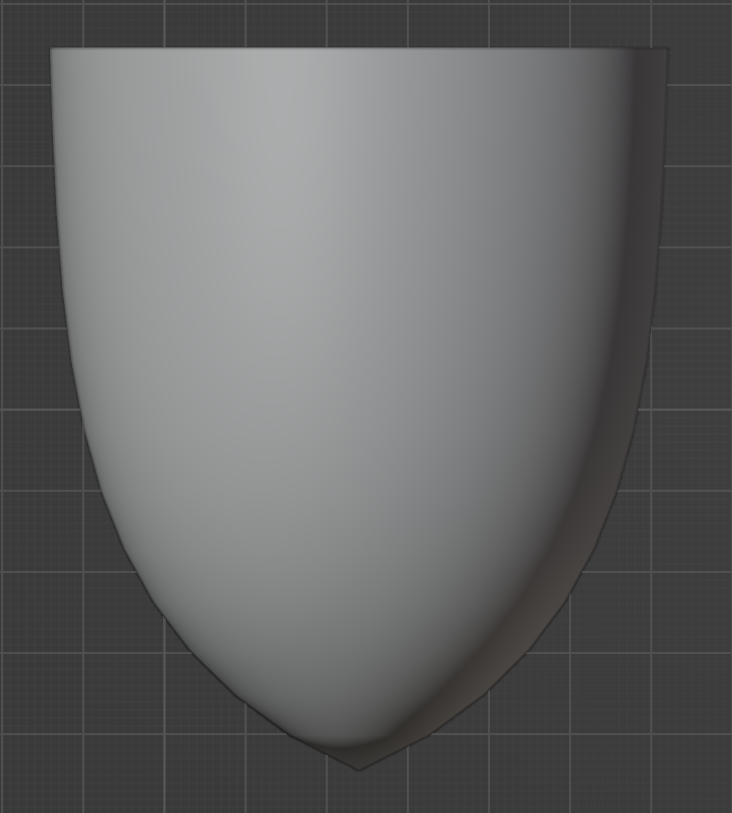
\includegraphics[width=.8\linewidth]{nose_5.png}
    \caption{Simulation targets 3 and 4}
    \label{fig:nose_5}
  \end{figure}

\chapter{Measurement Results}
\label{app:measurement_results}
  \begin{figure}[htbp]
    \centering
    \begin{subfigure}{.5\textwidth}
      \centering
      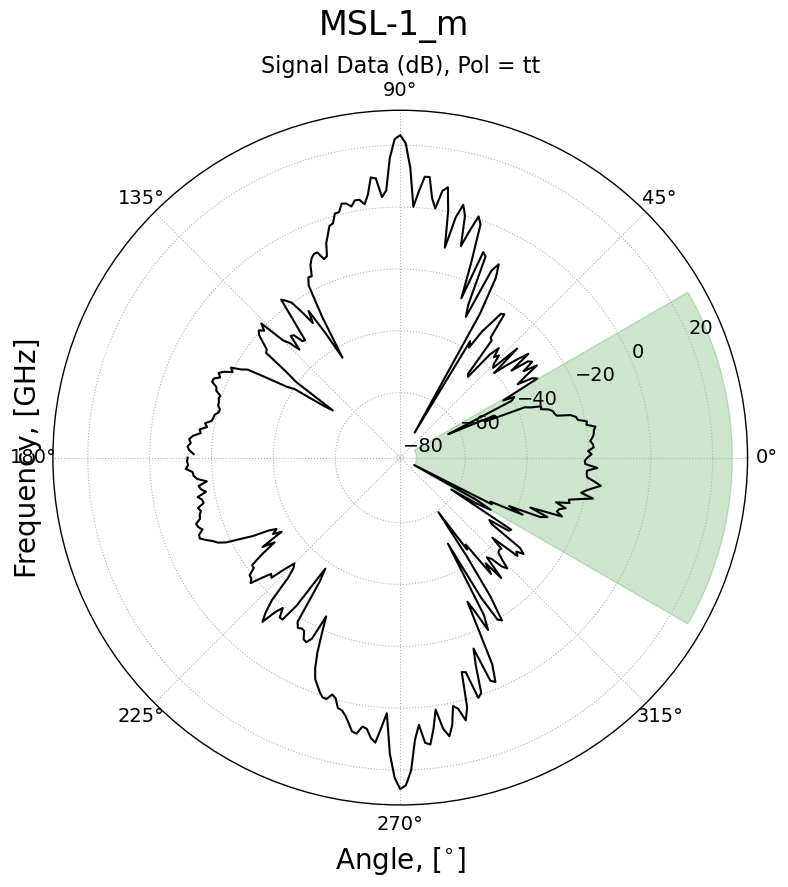
\includegraphics[width=.8\linewidth]{MSL-1_m_dB_tt_5GHz.png}
    \end{subfigure}%
    \begin{subfigure}{.5\textwidth}
      \centering
      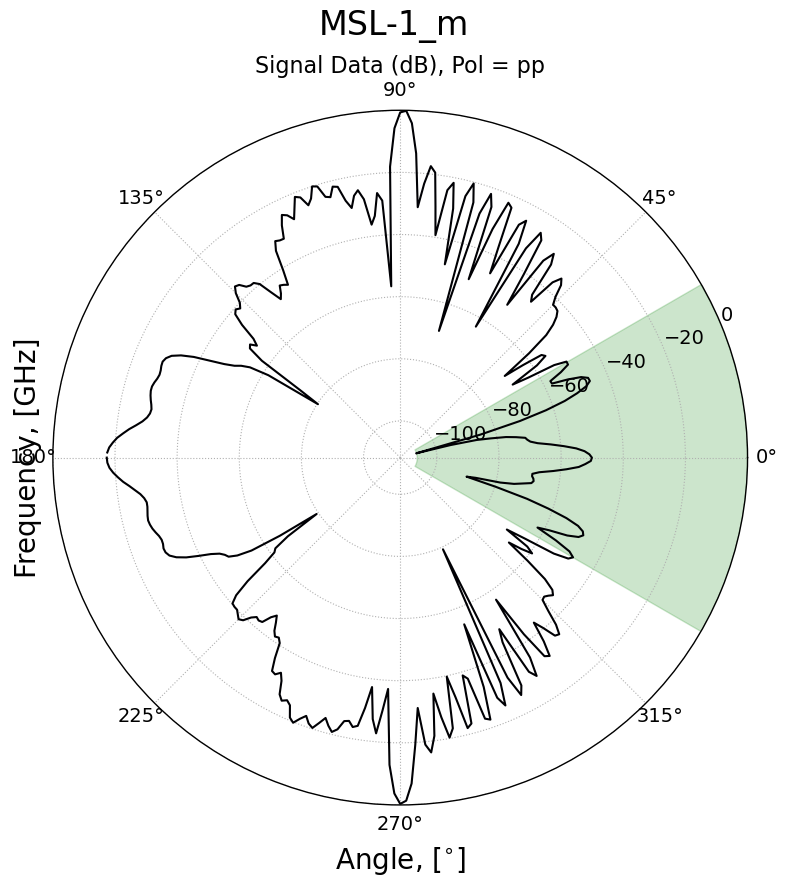
\includegraphics[width=.8\linewidth]{MSL-1_m_dB_pp_5GHz.png}
    \end{subfigure}
    \caption{Missile 1 \textcolor{green}{(Test)}:  RCS cut at 5 GHz. Vertical (tt) and Horizontal (pp) polarizations }
    \label{fig:n1}
  \end{figure}

  \begin{figure}[htbp]
    \centering
    \begin{subfigure}{.5\textwidth}
      \centering
      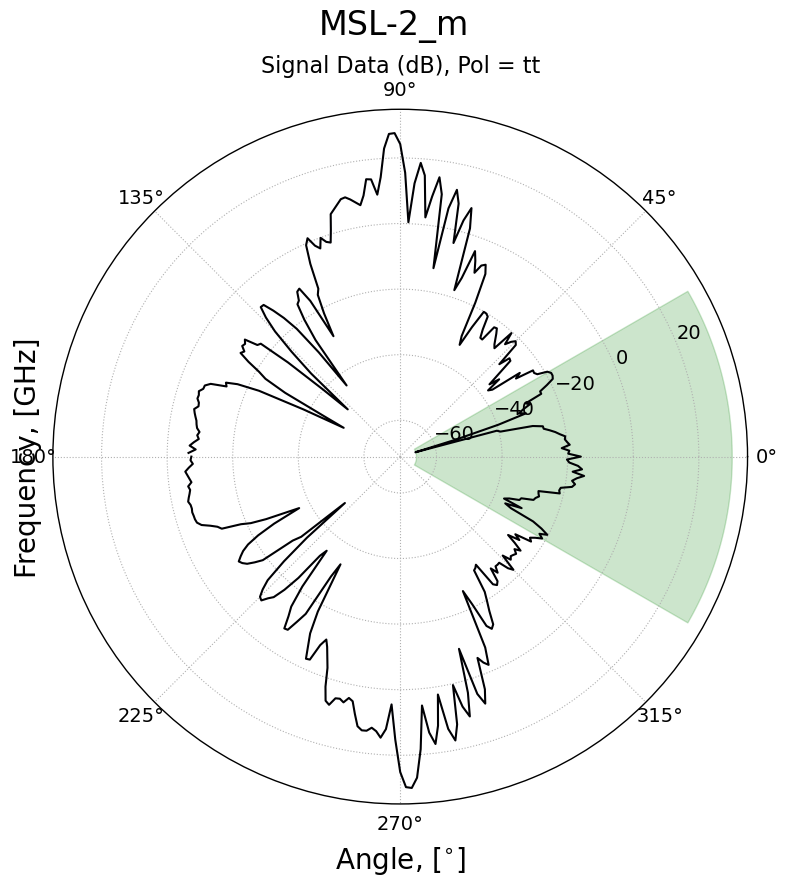
\includegraphics[width=.8\linewidth]{MSL-2_m_dB_tt_5GHz.png}
    \end{subfigure}%
    \begin{subfigure}{.5\textwidth}
      \centering
      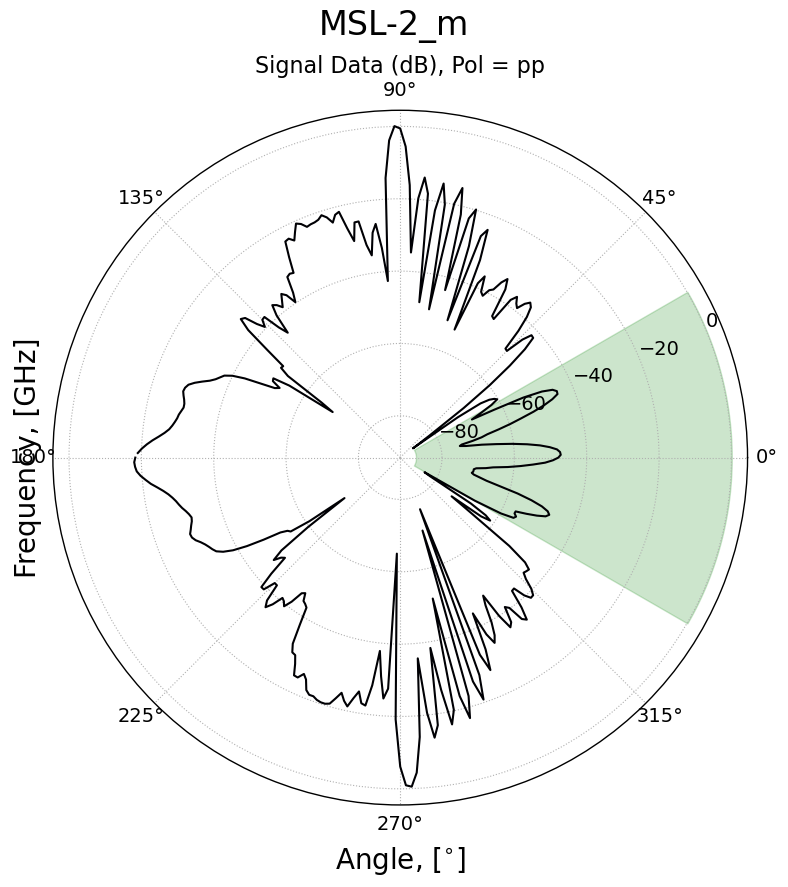
\includegraphics[width=.8\linewidth]{MSL-2_m_dB_pp_5GHz.png}
    \end{subfigure}
    \caption{Missile 2 \textcolor{green}{(Test)}:  RCS cut at 5 GHz. Vertical (tt) and Horizontal (pp) polarizations }
    \label{fig:n2}
  \end{figure}

  \begin{figure}[htbp]
    \centering
    \begin{subfigure}{.5\textwidth}
      \centering
      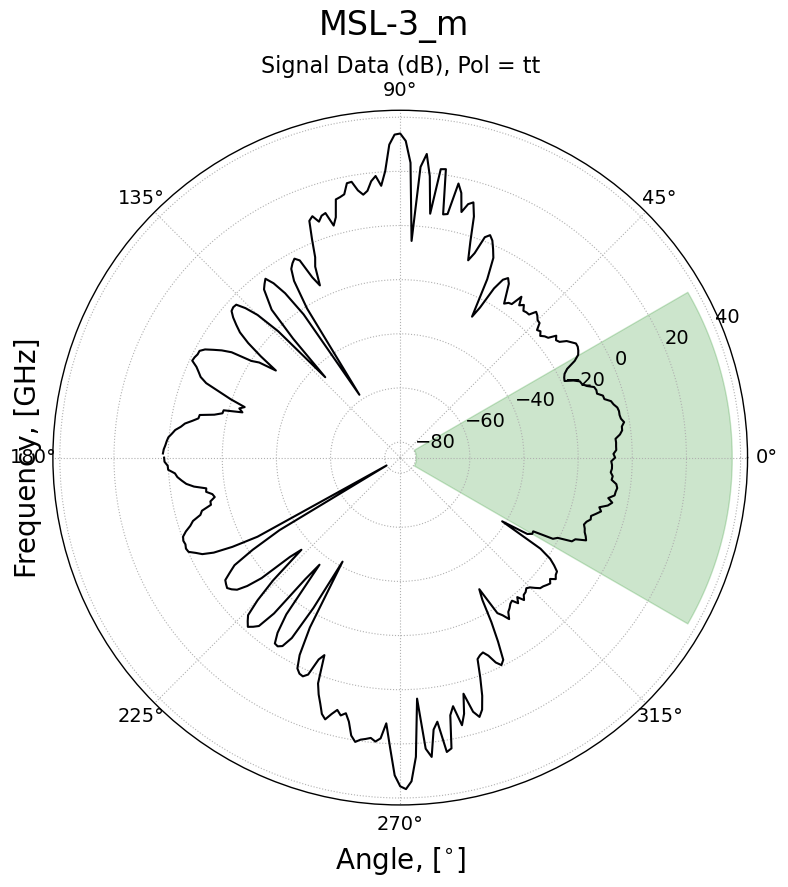
\includegraphics[width=.8\linewidth]{MSL-3_m_dB_tt_5GHz.png}
    \end{subfigure}%
    \begin{subfigure}{.5\textwidth}
      \centering
      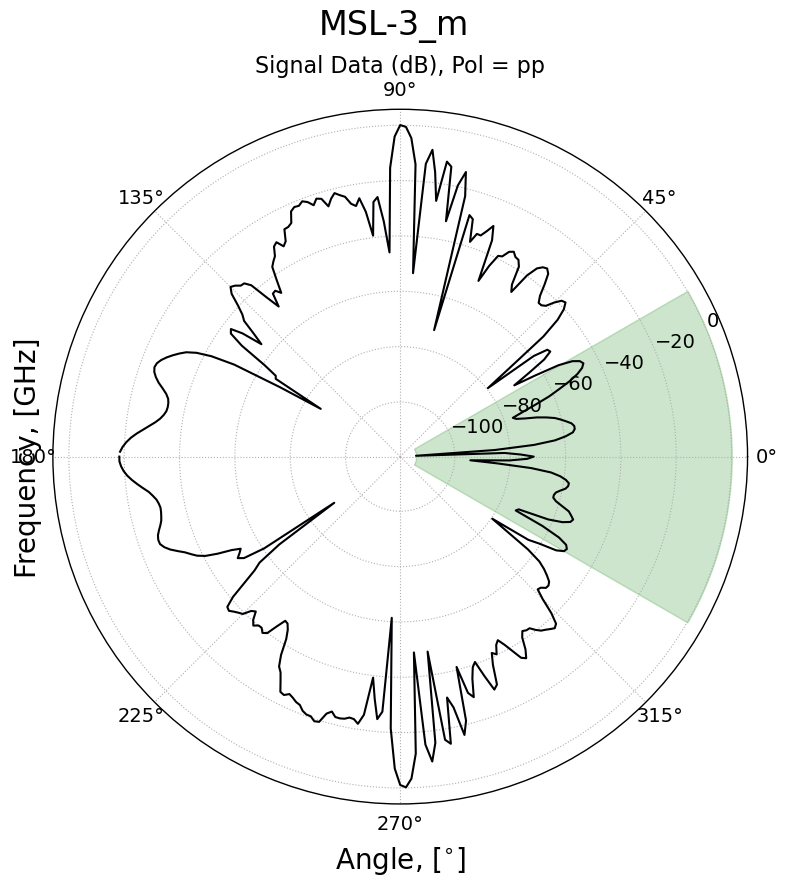
\includegraphics[width=.8\linewidth]{MSL-3_m_dB_pp_5GHz.png}
    \end{subfigure}
    \caption{Missile 3 \textcolor{green}{(Test)}:  RCS cut at 5 GHz. Vertical (tt) and Horizontal (pp) polarizations }
    \label{fig:n3}
  \end{figure}

  \begin{figure}[htbp]
    \centering
    \begin{subfigure}{.5\textwidth}
      \centering
      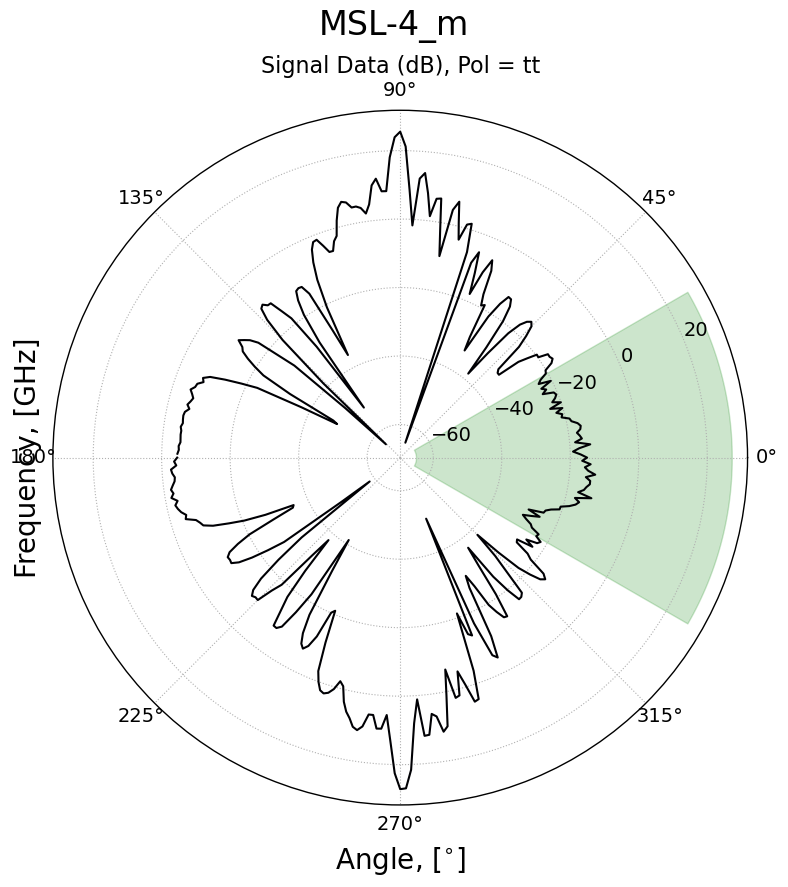
\includegraphics[width=.8\linewidth]{MSL-4_m_dB_tt_5GHz.png}
    \end{subfigure}%
    \begin{subfigure}{.5\textwidth}
      \centering
      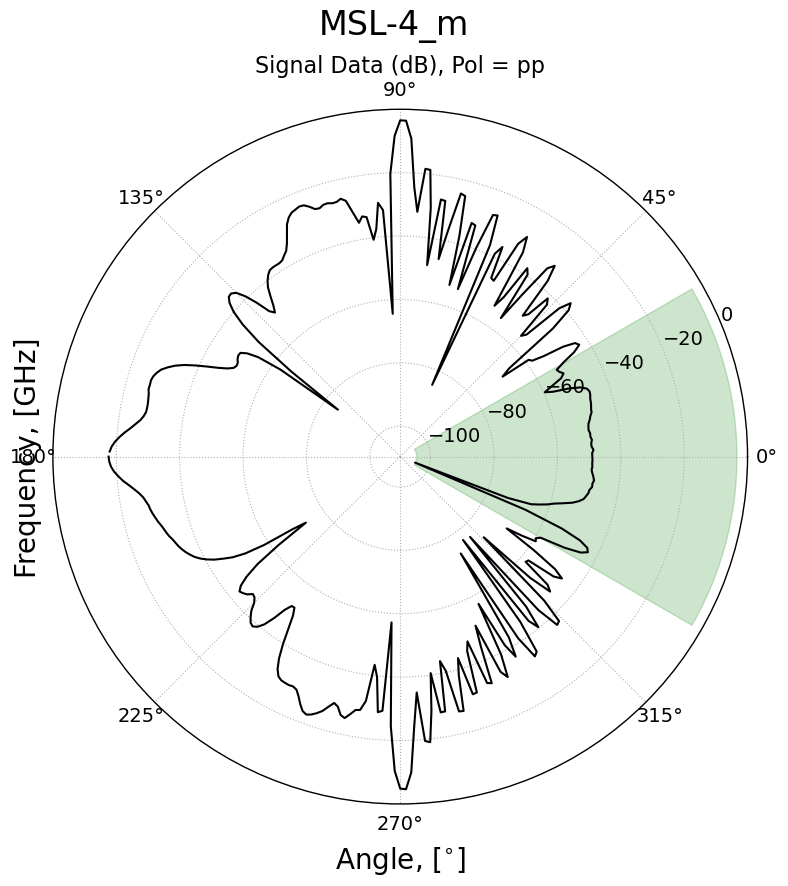
\includegraphics[width=.8\linewidth]{MSL-4_m_dB_pp_5GHz.png}
    \end{subfigure}
    \caption{Missile 4 \textcolor{green}{(Test)}:  RCS cut at 5 GHz. Vertical (tt) and Horizontal (pp) polarizations }
    \label{fig:n4}
  \end{figure}

  \begin{figure}[htbp]
    \centering
    \begin{subfigure}{.5\textwidth}
      \centering
      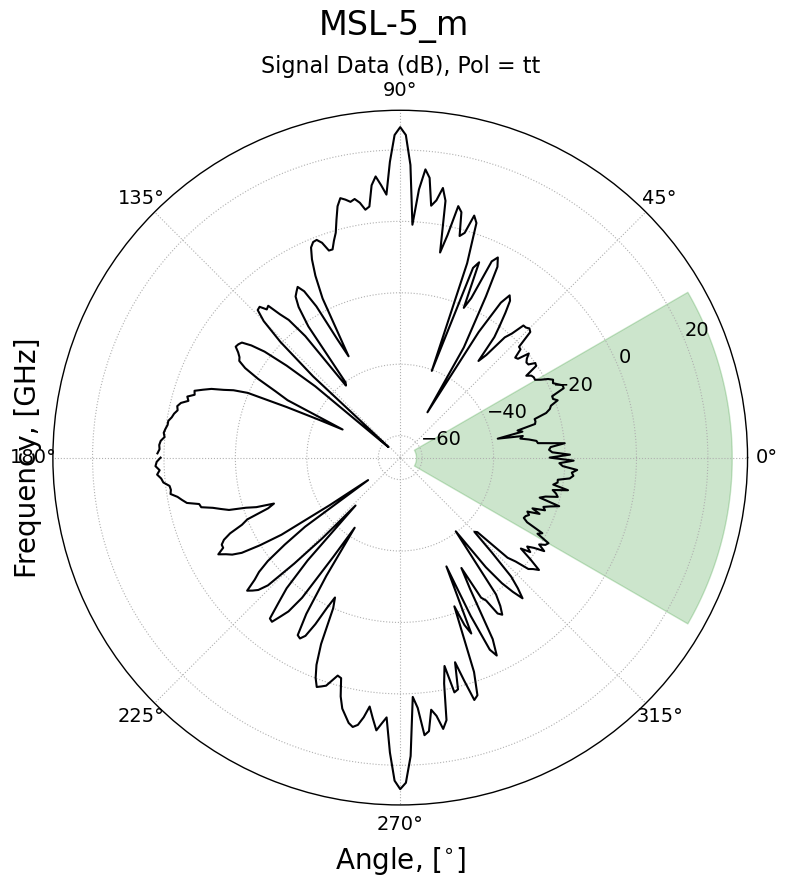
\includegraphics[width=.8\linewidth]{MSL-5_m_dB_tt_5GHz.png}
    \end{subfigure}%
    \begin{subfigure}{.5\textwidth}
      \centering
      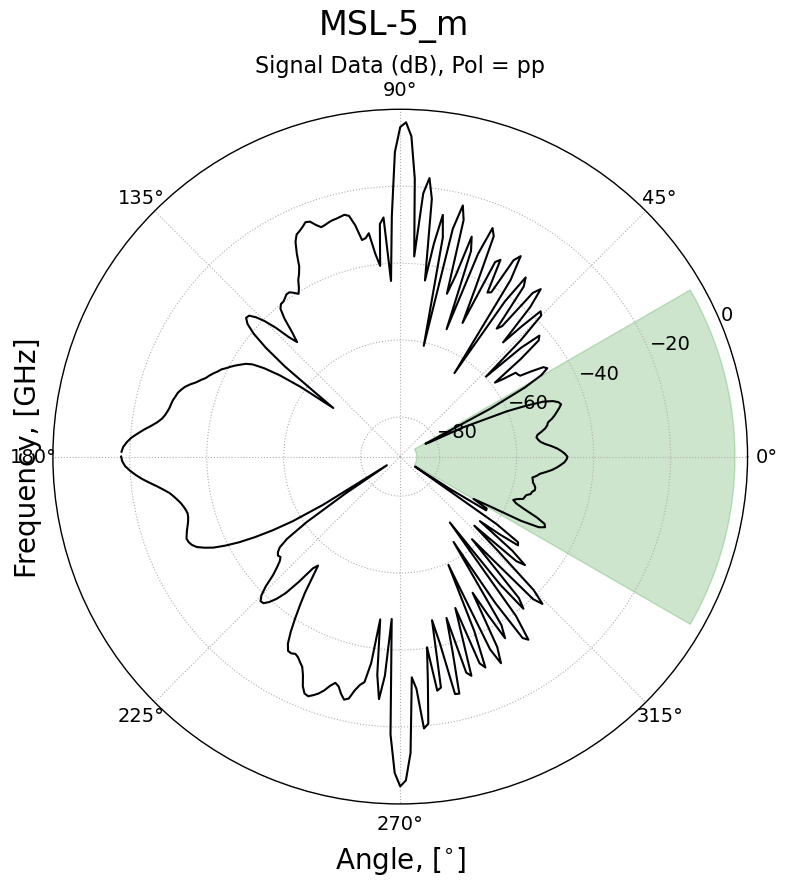
\includegraphics[width=.8\linewidth]{MSL-5_m_dB_pp_5GHz.png}
    \end{subfigure}
    \caption{Missile 5 \textcolor{green}{(Test)}:  RCS cut at 5 GHz. Vertical (tt) and Horizontal (pp) polarizations }
    \label{fig:n5}
  \end{figure}

  \begin{figure}[htbp]
    \centering
    \begin{subfigure}{.5\textwidth}
      \centering
      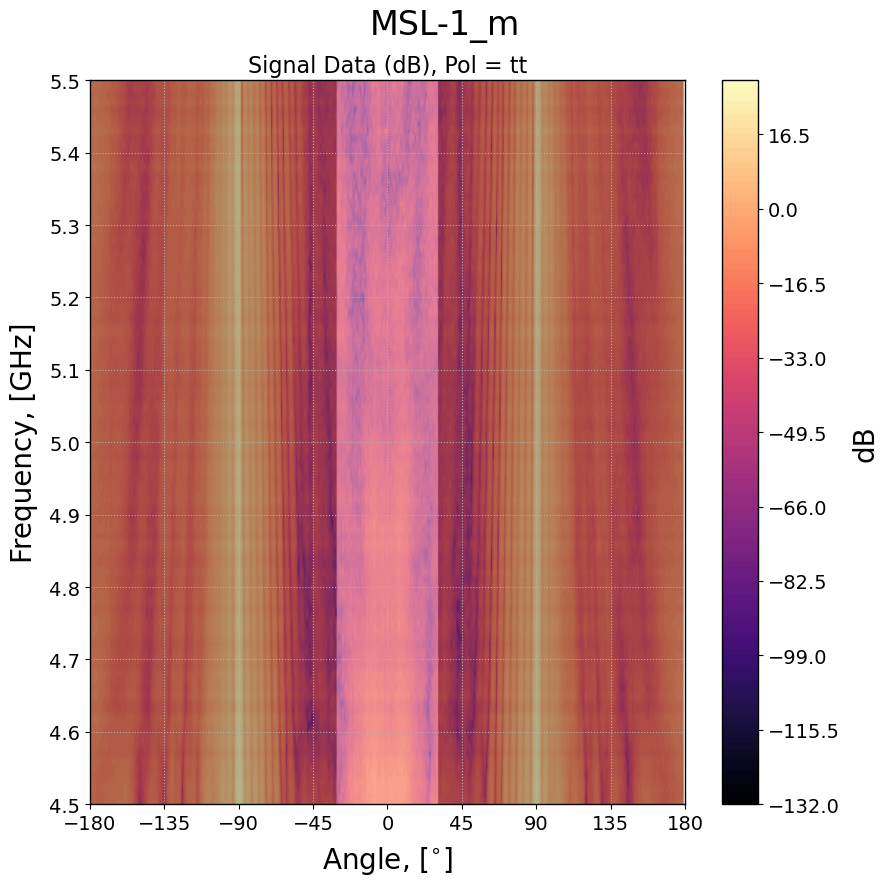
\includegraphics[width=.8\linewidth]{MSL-1_m_dB_tt.png}
    \end{subfigure}%
    \begin{subfigure}{.5\textwidth}
      \centering
      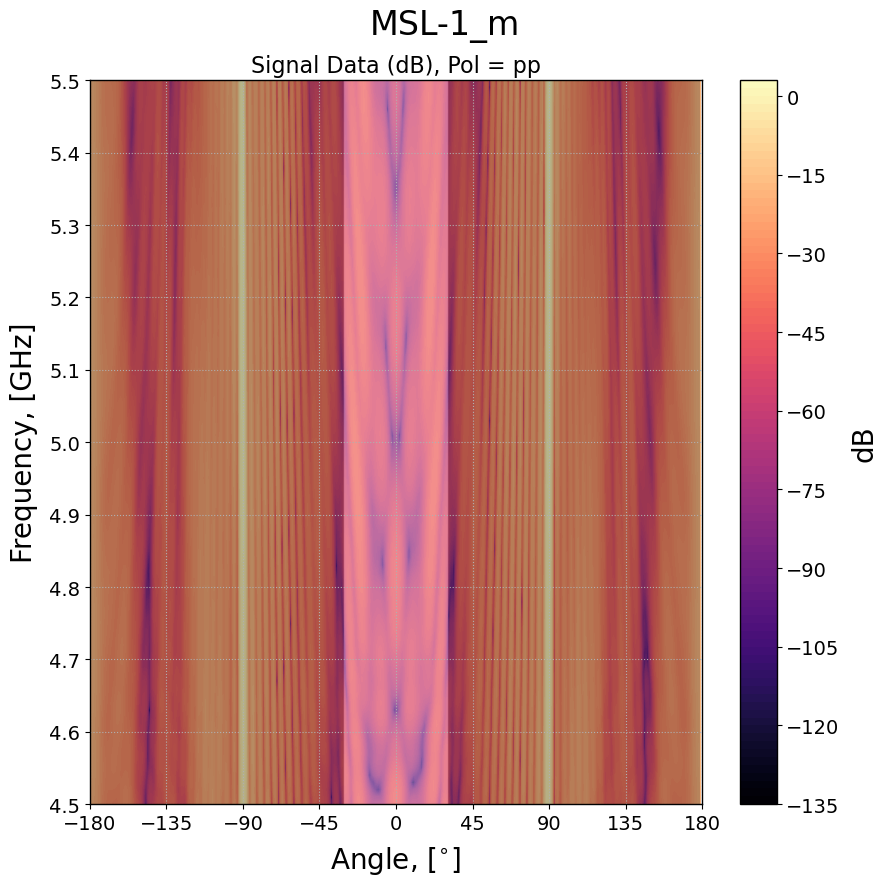
\includegraphics[width=.8\linewidth]{MSL-1_m_dB_pp.png}
    \end{subfigure}
    \caption{Missile 1 \textcolor{green}{(Test)}:  Total RCS. Vertical (tt) and Horizontal (pp) polarizations }
    \label{fig:c1}
  \end{figure}

  \begin{figure}[htbp]
    \centering
    \begin{subfigure}{.5\textwidth}
      \centering
      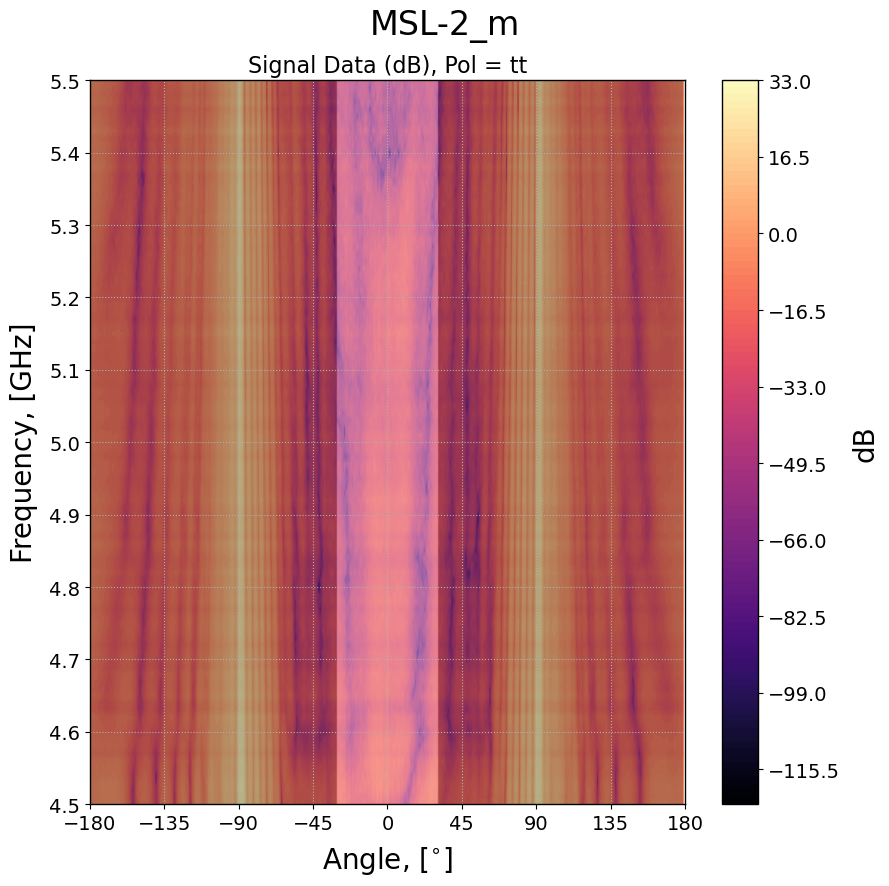
\includegraphics[width=.8\linewidth]{MSL-2_m_dB_tt.png}
    \end{subfigure}%
    \begin{subfigure}{.5\textwidth}
      \centering
      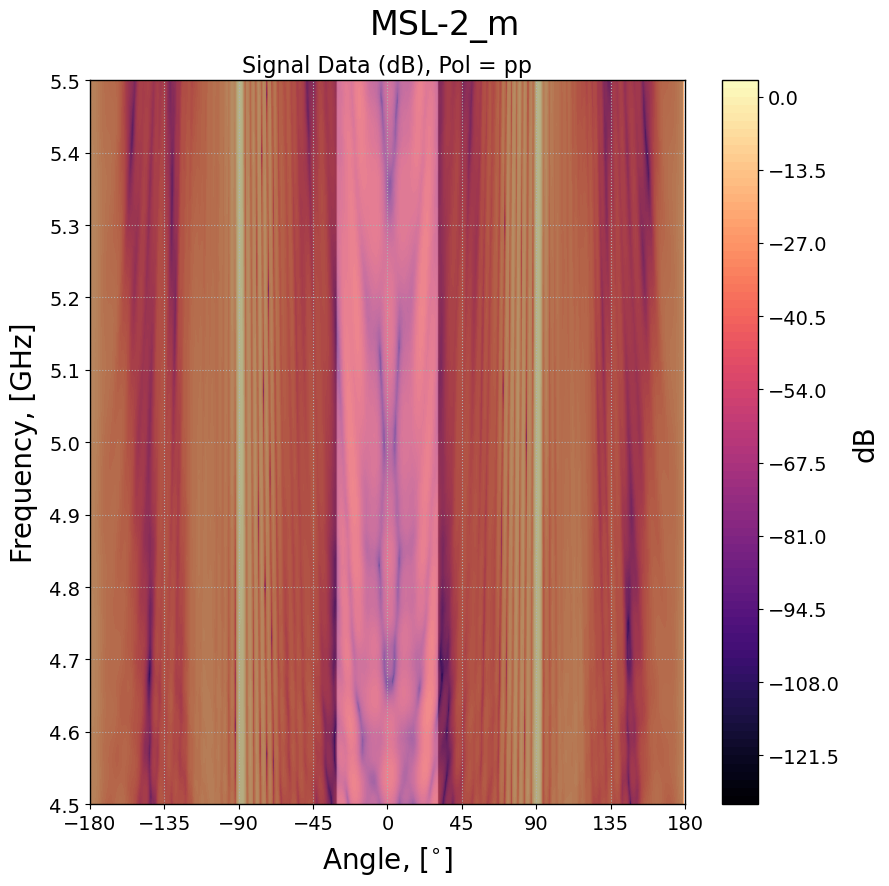
\includegraphics[width=.8\linewidth]{MSL-2_m_dB_pp.png}
    \end{subfigure}
    \caption{Missile 2 \textcolor{green}{(Test)}:  Total RCS. Vertical (tt) and Horizontal (pp) polarizations }
    \label{fig:c2}
  \end{figure}

  \begin{figure}[htbp]
    \centering
    \begin{subfigure}{.5\textwidth}
      \centering
      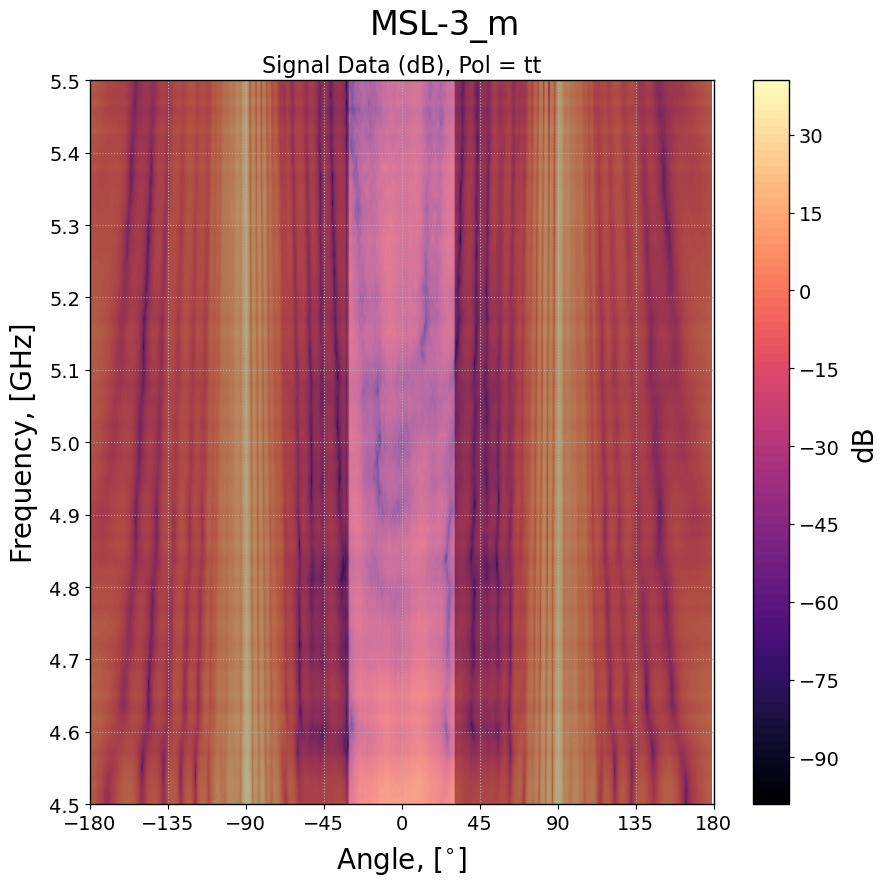
\includegraphics[width=.8\linewidth]{MSL-3_m_dB_tt.png}
    \end{subfigure}%
    \begin{subfigure}{.5\textwidth}
      \centering
      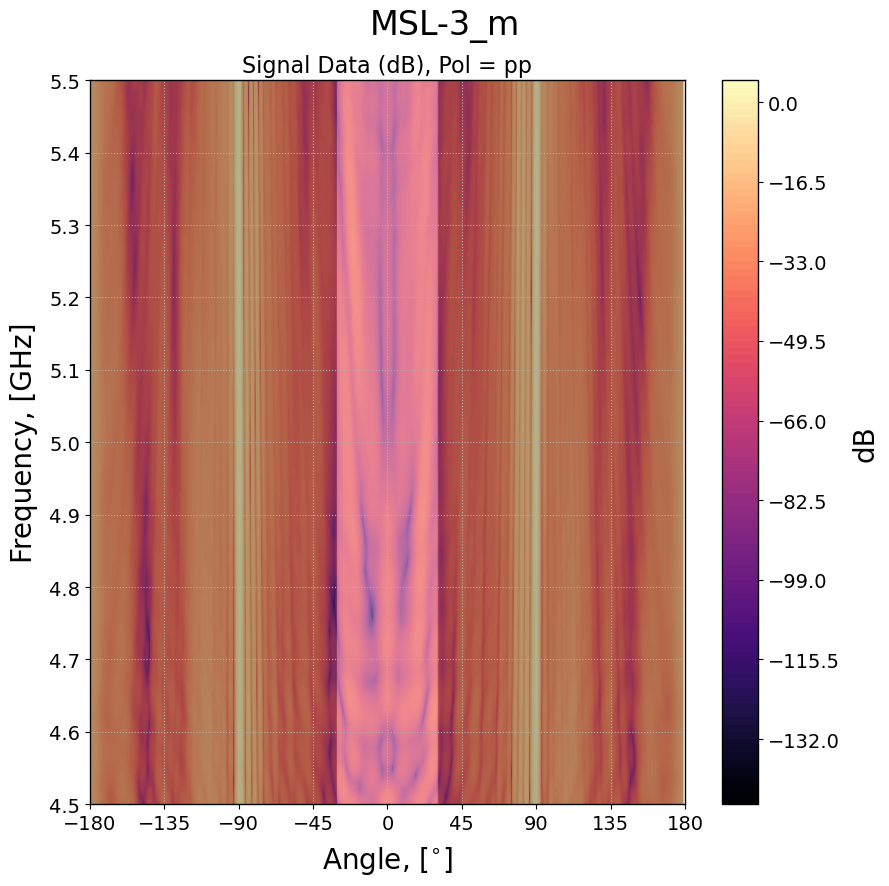
\includegraphics[width=.8\linewidth]{MSL-3_m_dB_pp.png}
    \end{subfigure}
    \caption{Missile 3 \textcolor{green}{(Test)}:  Total RCS. Vertical (tt) and Horizontal (pp) polarizations }
    \label{fig:c3}
  \end{figure}

  \begin{figure}[htbp]
    \centering
    \begin{subfigure}{.5\textwidth}
      \centering
      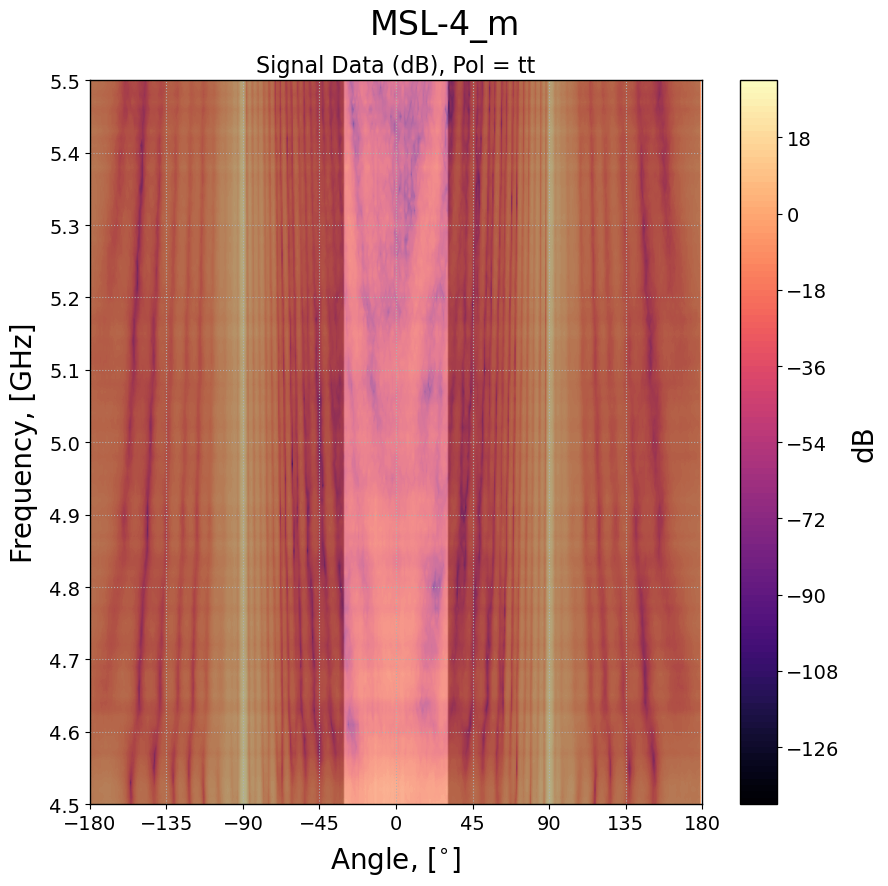
\includegraphics[width=.8\linewidth]{MSL-4_m_dB_tt.png}
    \end{subfigure}%
    \begin{subfigure}{.5\textwidth}
      \centering
      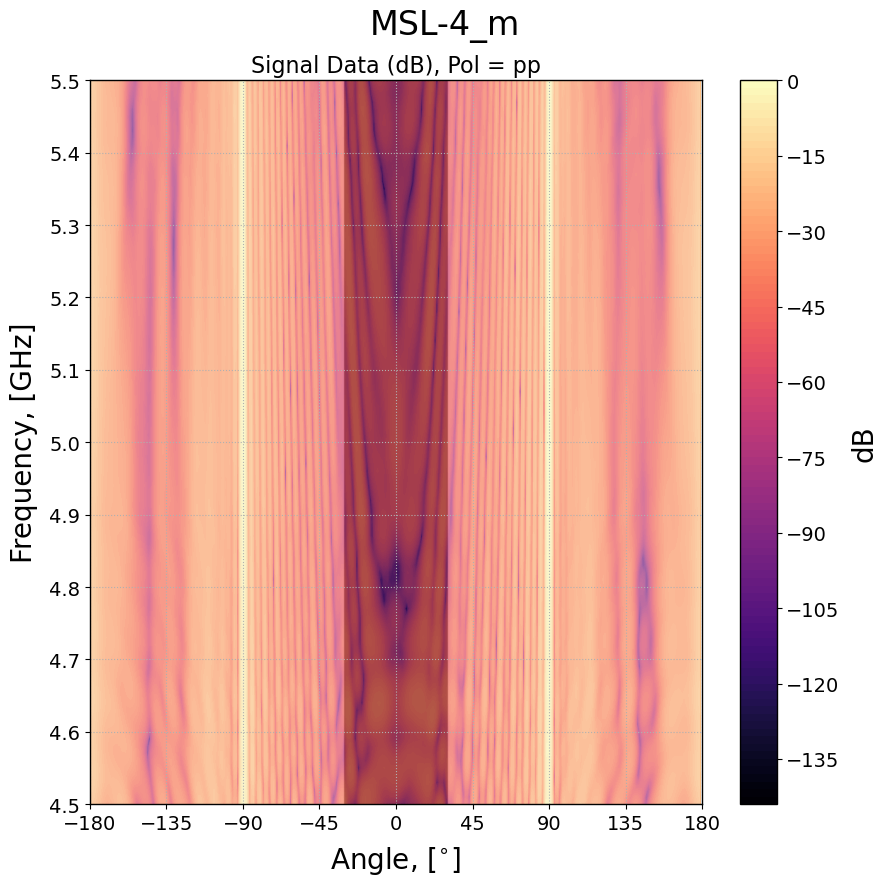
\includegraphics[width=.8\linewidth]{MSL-4_m_dB_pp.png}
    \end{subfigure}
    \caption{Missile 4 \textcolor{green}{(Test)}:  Total RCS. Vertical (tt) and Horizontal (pp) polarizations }
    \label{fig:c4}
  \end{figure}

  \begin{figure}[htbp]
    \centering
    \begin{subfigure}{.5\textwidth}
      \centering
      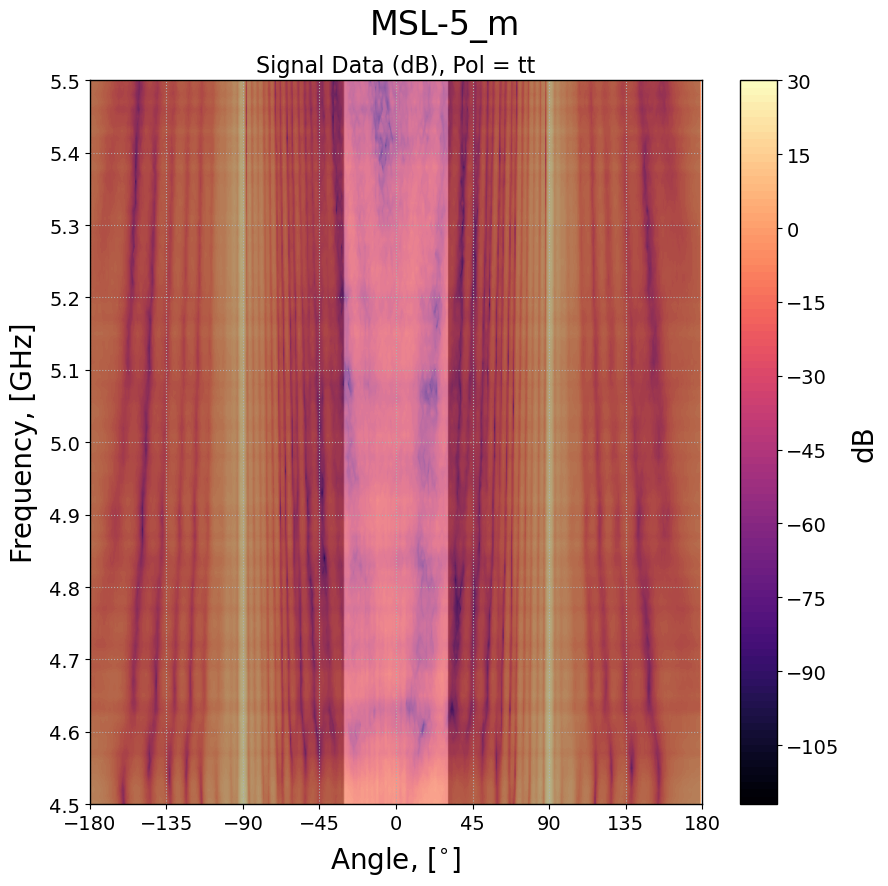
\includegraphics[width=.8\linewidth]{MSL-5_m_dB_tt.png}
    \end{subfigure}%
    \begin{subfigure}{.5\textwidth}
      \centering
      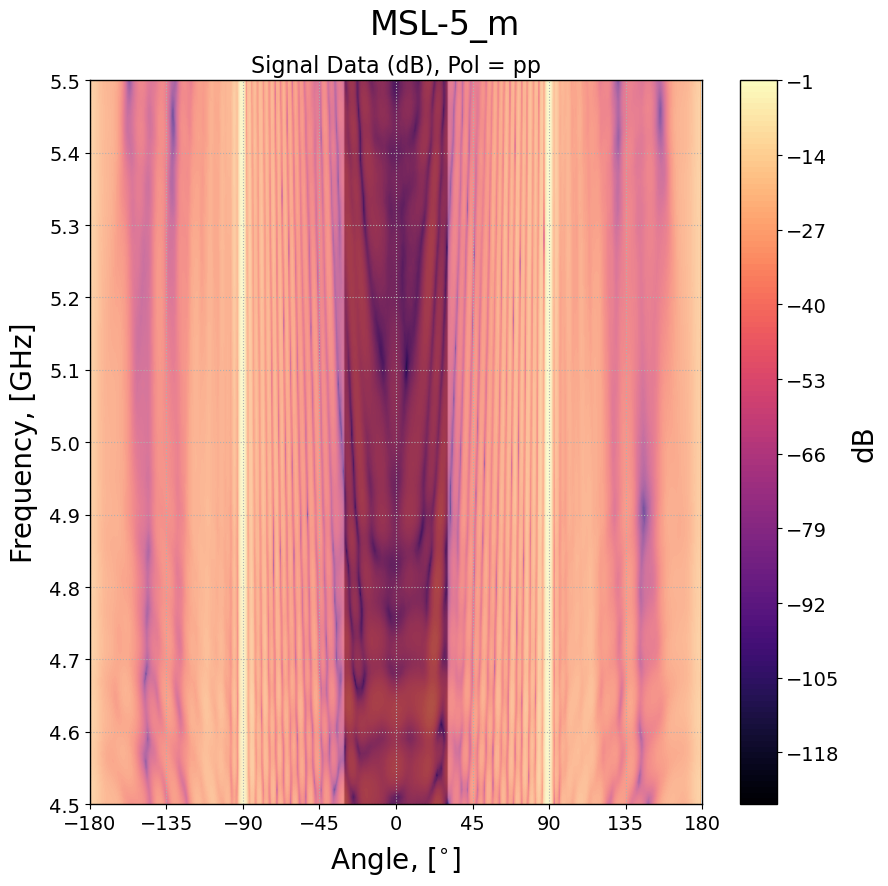
\includegraphics[width=.8\linewidth]{MSL-5_m_dB_pp.png}
    \end{subfigure}
    \caption{Missile 5 \textcolor{green}{(Test)}:  Total RCS. Vertical (tt) and Horizontal (pp) polarizations }
    \label{fig:c5}
  \end{figure}

\chapter{Simulation Results}
\label{app:simulation_results}
  \begin{figure}[htbp]
    \centering
    \begin{subfigure}{.5\textwidth}
      \centering
      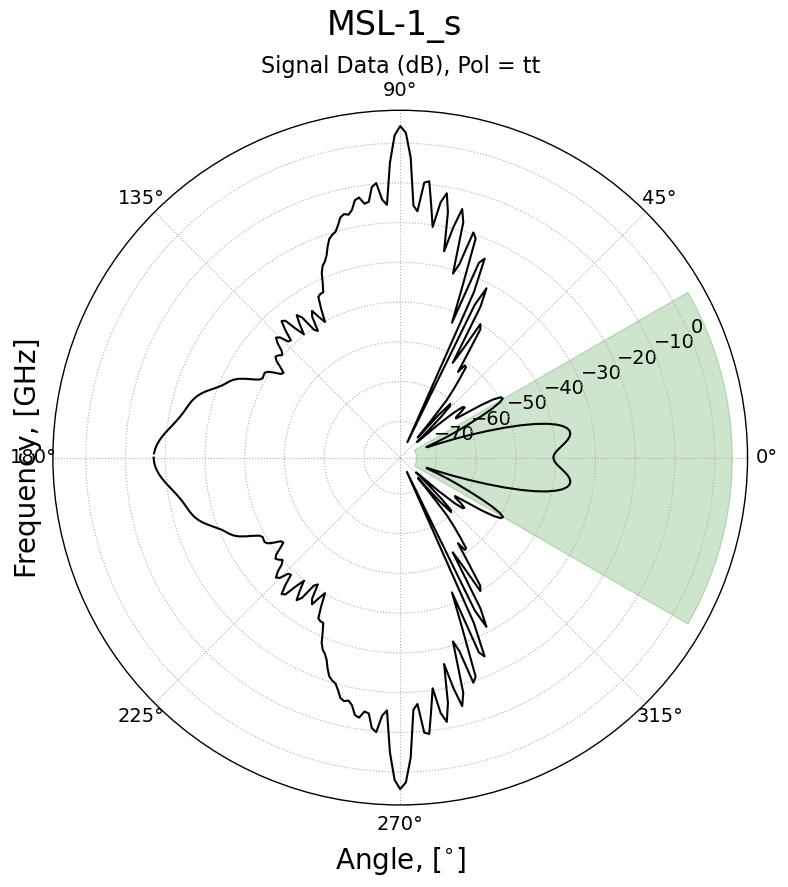
\includegraphics[width=.8\linewidth]{MSL-1_s_dB_tt_5GHz.png}
    \end{subfigure}%
    \begin{subfigure}{.5\textwidth}
      \centering
      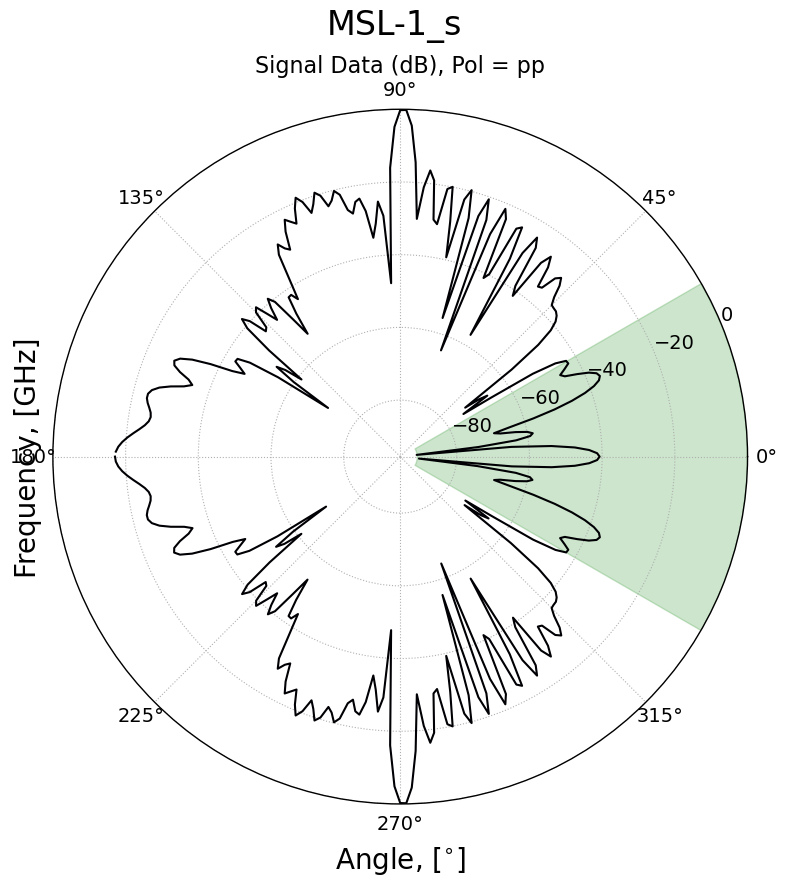
\includegraphics[width=.8\linewidth]{MSL-1_s_dB_pp_5GHz.png}
    \end{subfigure}
    \caption{Missile 1 \textcolor{red}{(Sim)}:  RCS cut at 5 GHz. Vertical (tt) and Horizontal (pp) polarizations }
    \label{fig:ns1}
  \end{figure}

  \begin{figure}[htbp]
    \centering
    \begin{subfigure}{.5\textwidth}
      \centering
      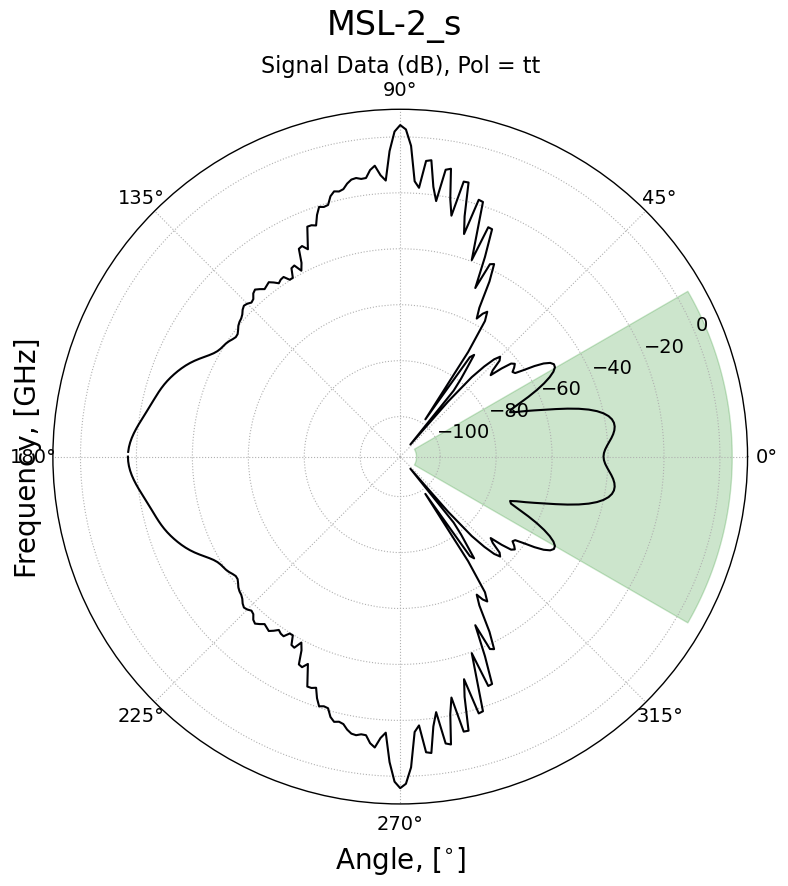
\includegraphics[width=.8\linewidth]{MSL-2_s_dB_tt_5GHz.png}
    \end{subfigure}%
    \begin{subfigure}{.5\textwidth}
      \centering
      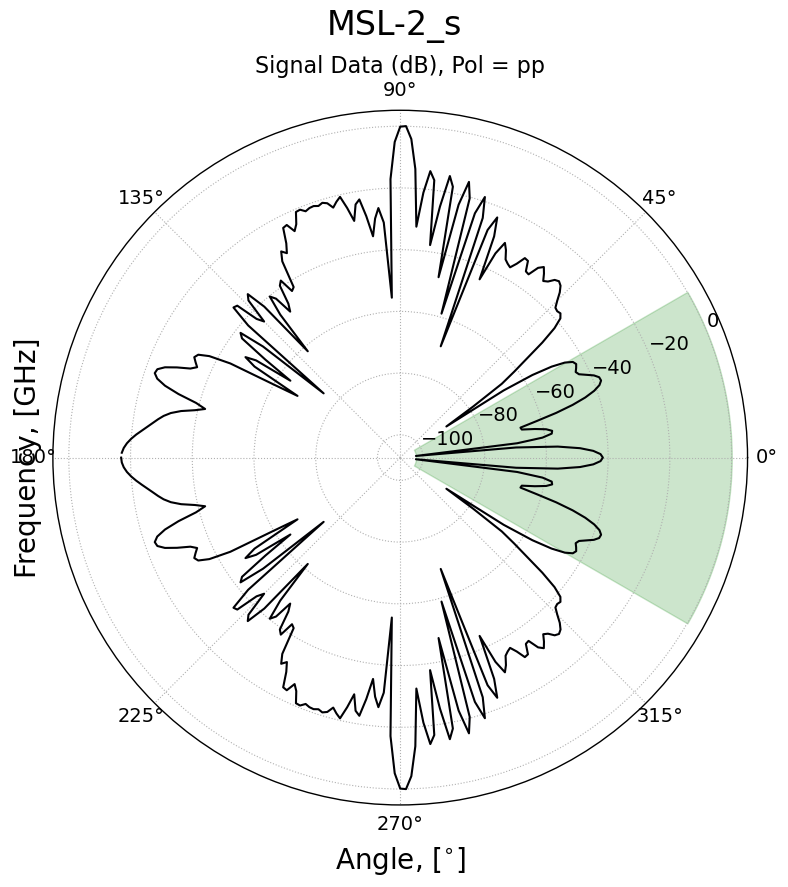
\includegraphics[width=.8\linewidth]{MSL-2_s_dB_pp_5GHz.png}
    \end{subfigure}
    \caption{Missile 2 \textcolor{red}{(Sim)}:  RCS cut at 5 GHz. Vertical (tt) and Horizontal (pp) polarizations }
    \label{fig:ns2}
  \end{figure}

  \begin{figure}[htbp]
    \centering
    \begin{subfigure}{.5\textwidth}
      \centering
      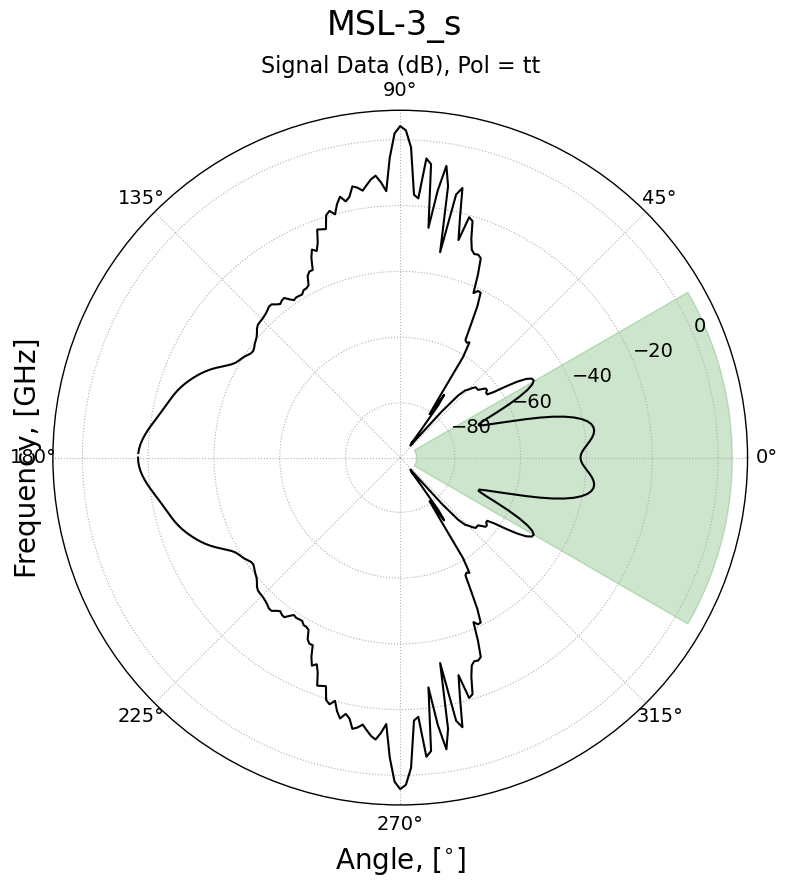
\includegraphics[width=.8\linewidth]{MSL-3_s_dB_tt_5GHz.png}
    \end{subfigure}%
    \begin{subfigure}{.5\textwidth}
      \centering
      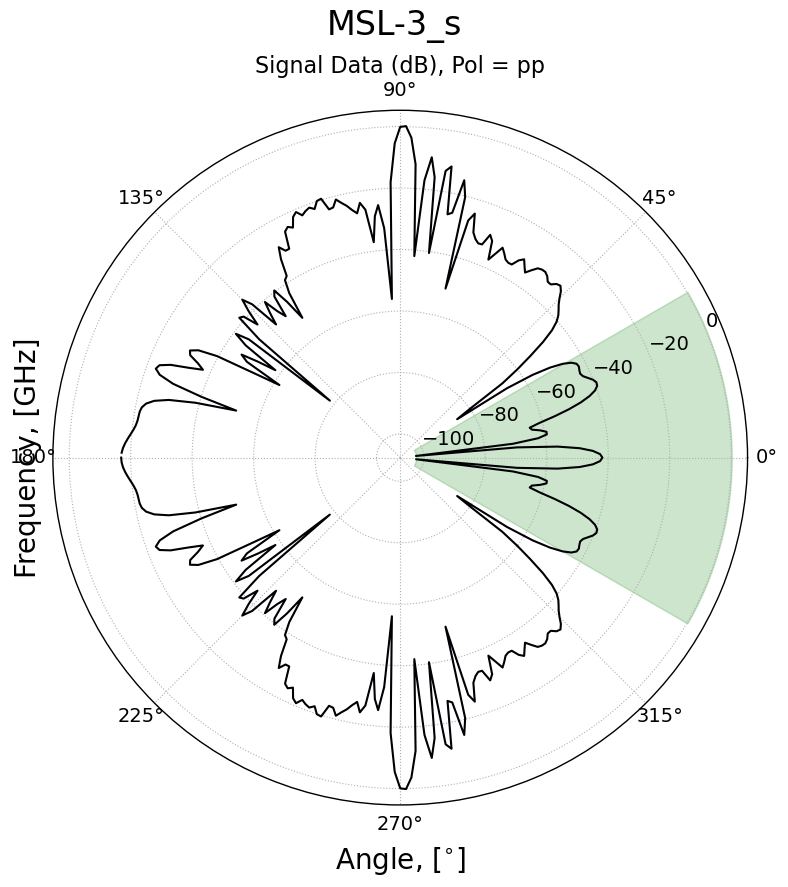
\includegraphics[width=.8\linewidth]{MSL-3_s_dB_pp_5GHz.png}
    \end{subfigure}
    \caption{Missile 3 \textcolor{red}{(Sim)}:  RCS cut at 5 GHz. Vertical (tt) and Horizontal (pp) polarizations }
    \label{fig:ns3}
  \end{figure}

  \begin{figure}[htbp]
    \centering
    \begin{subfigure}{.5\textwidth}
      \centering
      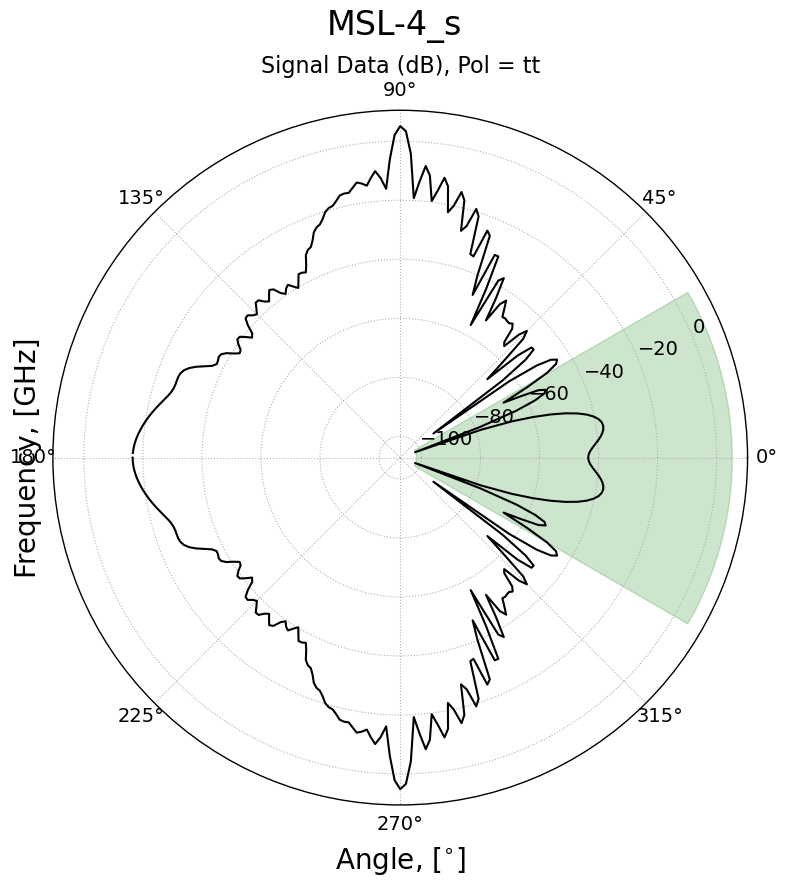
\includegraphics[width=.8\linewidth]{MSL-4_s_dB_tt_5GHz.png}
    \end{subfigure}%
    \begin{subfigure}{.5\textwidth}
      \centering
      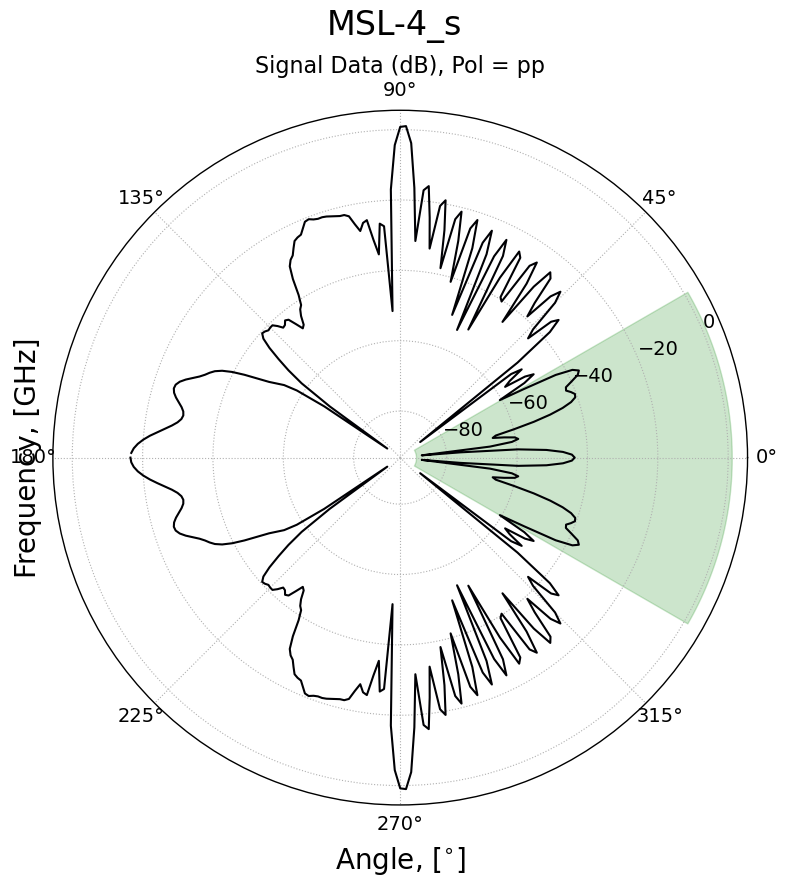
\includegraphics[width=.8\linewidth]{MSL-4_s_dB_pp_5GHz.png}
    \end{subfigure}
    \caption{Missile 4 \textcolor{red}{(Sim)}:  RCS cut at 5 GHz. Vertical (tt) and Horizontal (pp) polarizations }
    \label{fig:ns4}
  \end{figure}

  \begin{figure}[htbp]
    \centering
    \begin{subfigure}{.5\textwidth}
      \centering
      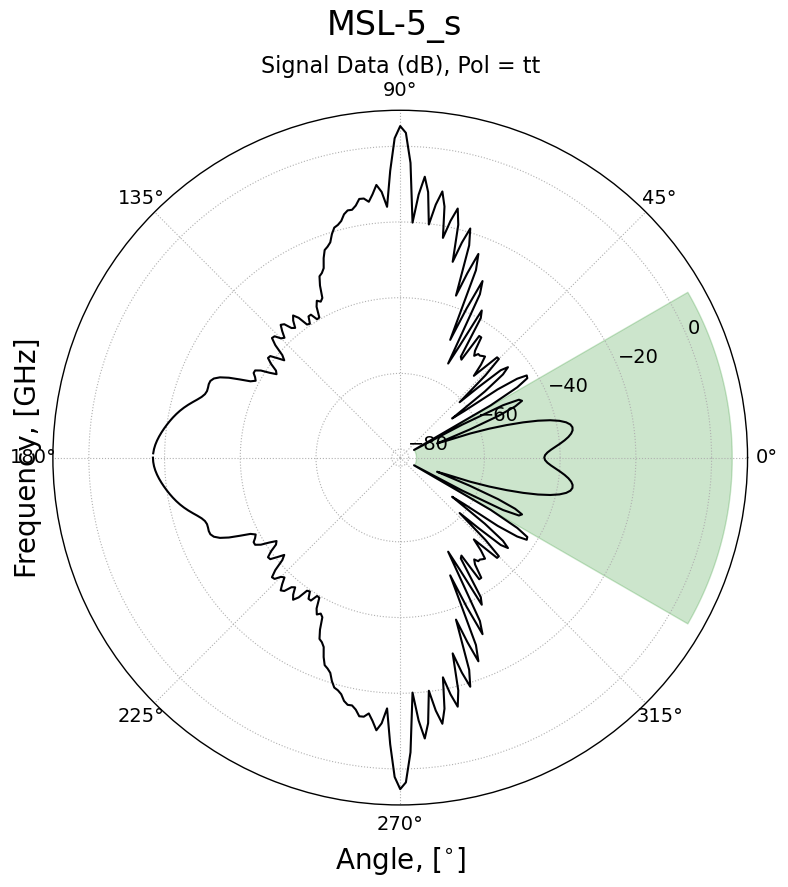
\includegraphics[width=.8\linewidth]{MSL-5_s_dB_tt_5GHz.png}
    \end{subfigure}%
    \begin{subfigure}{.5\textwidth}
      \centering
      \includegraphics[width=.8\linewidth]{MSL-5_s_dB_pp_5GHz.png}
    \end{subfigure}
    \caption{Missile 5 \textcolor{red}{(Sim)}:  RCS cut at 5 GHz. Vertical (tt) and Horizontal (pp) polarizations }
    \label{fig:ns5}
  \end{figure}

\chapter{Correlation Results}
\label{app:correlation_results}
  \begin{figure}[htbp!]
    \centering
    \includegraphics[width=.9\linewidth]{Corr_SNR_MSL-1_s_Nfs.png}
    \caption[Missile 1 Correlations (Sim/Meas)]{Correlation between the simulation of missile 1, and the measured RCS values for each target.}
    \label{fig:corr_msl1}
  \end{figure}

  \begin{figure}[htbp!]
    \centering
    \includegraphics[width=.9\linewidth]{Corr_SNR_MSL-2_s_Nfs.png}
    \caption[Missile 1 Correlations (Sim/Meas)]{Correlation between the simulation of missile 2, and the measured RCS values for each target.}
    \label{fig:corr_msl2}
  \end{figure}

  \begin{figure}[htbp!]
    \centering
    \includegraphics[width=.9\linewidth]{Corr_SNR_MSL-3_s_Nfs.png}
    \caption[Missile 1 Correlations (Sim/Meas)]{Correlation between the simulation of missile 3, and the measured RCS values for each target.}
    \label{fig:corr_msl3}
  \end{figure}

  \begin{figure}[htbp!]
    \centering
    \includegraphics[width=.9\linewidth]{Corr_SNR_MSL-4_s_Nfs.png}
    \caption[Missile 1 Correlations (Sim/Meas)]{Correlation between the simulation of missile 4, and the measured RCS values for each target.}
    \label{fig:corr_msl4}
  \end{figure}

  \begin{figure}[htbp!]
    \centering
    \includegraphics[width=.9\linewidth]{Corr_SNR_MSL-5_s_Nfs.png}
    \caption[Missile 1 Correlations (Sim/Sim)]{Correlation between the simulation of missile 5, and the measured RCS values for each target.}
    \label{fig:corr_msl5}
  \end{figure}

  \begin{figure}[htbp!]
    \centering
    \includegraphics[width=.9\linewidth]{vgg-19_sim_Corr_SNR_MSL-1_s_Nfs.png}
    \caption[Missile 1 Correlations (Sim/Sim)]{Correlation between the simulation of missile 1, and the simulated RCS values for each target.}
    \label{fig:corr_msl1_sim}
  \end{figure}

  \begin{figure}[htbp!]
    \centering
    \includegraphics[width=.9\linewidth]{vgg-19_sim_Corr_SNR_MSL-2_s_Nfs.png}
    \caption[Missile 1 Correlations (Sim/Sim)]{Correlation between the simulation of missile 2, and the simulated RCS values for each target.}
    \label{fig:corr_msl2_sim}
  \end{figure}

  \begin{figure}[htbp!]
    \centering
    \includegraphics[width=.9\linewidth]{vgg-19_sim_Corr_SNR_MSL-3_s_Nfs.png}
    \caption[Missile 1 Correlations (Sim/Sim)]{Correlation between the simulation of missile 3, and the simulated RCS values for each target.}
    \label{fig:corr_msl3_sim}
  \end{figure}

  \begin{figure}[htbp!]
    \centering
    \includegraphics[width=.9\linewidth]{vgg-19_sim_Corr_SNR_MSL-4_s_Nfs.png}
    \caption[Missile 1 Correlations (Sim/Sim)]{Correlation between the simulation of missile 4, and the simulated RCS values for each target.}
    \label{fig:corr_msl4_sim}
  \end{figure}

  \begin{figure}[htbp!]
    \centering
    \includegraphics[width=.9\linewidth]{vgg-19_sim_Corr_SNR_MSL-5_s_Nfs.png}
    \caption[Missile 1 Correlations (Sim/Sim)]{Correlation between the simulation of missile 5, and the simulated RCS values for each target.}
    \label{fig:corr_msl5_sim}
  \end{figure}

\chapter{VGG-19 Results}
\label{app:vgg-19_results}

  \begin{figure}[htbp!]
    \centering
    \includegraphics[width=.9\linewidth]{19_1_CM.png}
    \caption[VGG-19, -10 dBm Confusion Matrix]{Confusion matrix for the -10 dBm model in the VGG-19 siamese network.}
    \label{fig:vgg-19_cm1}
  \end{figure}

  \begin{figure}[htbp!]
    \centering
    \includegraphics[width=.9\linewidth]{19_2_CM.png}
    \caption[VGG-19, -5 dBm Confusion Matrix]{Confusion matrix for the -5 dBm model in the VGG-19 siamese network.}
    \label{fig:vgg-19_cm2}
  \end{figure}

  \begin{figure}[htbp!]
    \centering
    \includegraphics[width=.9\linewidth]{19_3_CM.png}
    \caption[VGG-19, 0 dBm Confusion Matrix]{Confusion matrix for the 0 dBm model in the VGG-19 siamese network.}
    \label{fig:vgg-19_cm3}
  \end{figure}

  \begin{figure}[htbp!]
    \centering
    \includegraphics[width=.9\linewidth]{19_4_CM.png}
    \caption[VGG-19, 5 dBm Confusion Matrix]{Confusion matrix for the 5 dBm model in the VGG-19 siamese network.}
    \label{fig:vgg-19_cm4}
  \end{figure}

  \begin{figure}[htbp!]
    \centering
    \includegraphics[width=.9\linewidth]{19_5_CM.png}
    \caption[VGG-19, 10 dBm Confusion Matrix]{Confusion matrix for the 10 dBm model in the VGG-19 siamese network.}
    \label{fig:vgg-19_cm5}
  \end{figure}

  \begin{figure}[htbp]
    \centering
    \begin{subfigure}{.5\textwidth}
      \centering
      \includegraphics[width=.9\linewidth]{vgg-19_meas_Angle_ACC_-10.png}
    \end{subfigure}%
    \begin{subfigure}{.5\textwidth}
      \centering
      \includegraphics[width=.9\linewidth]{vgg-19_meas_Pred_Angle_-10.png}
    \end{subfigure}
    \caption{Angle accuracy and Classification for the VGG-19 siamese network, SNR=-10 dB}
    \label{fig:vgg-19_snr1}
  \end{figure}

  \begin{figure}[htbp]
    \centering
    \begin{subfigure}{.5\textwidth}
      \centering
      \includegraphics[width=.9\linewidth]{vgg-19_meas_Angle_ACC_-8.png}
    \end{subfigure}%
    \begin{subfigure}{.5\textwidth}
      \centering
      \includegraphics[width=.9\linewidth]{vgg-19_meas_Pred_Angle_-8.png}
    \end{subfigure}
    \caption{Angle accuracy and Classification for the VGG-19 siamese network, SNR=-8 dB}
    \label{fig:vgg-19_snr2}
  \end{figure}

  \begin{figure}[htbp]
    \centering
    \begin{subfigure}{.5\textwidth}
      \centering
      \includegraphics[width=.9\linewidth]{vgg-19_meas_Angle_ACC_-6.png}
    \end{subfigure}%
    \begin{subfigure}{.5\textwidth}
      \centering
      \includegraphics[width=.9\linewidth]{vgg-19_meas_Pred_Angle_-6.png}
    \end{subfigure}
    \caption{Angle accuracy and Classification for the VGG-19 siamese network, SNR=-6 dB}
    \label{fig:vgg-19_snr3}
  \end{figure}

  \begin{figure}[htbp]
    \centering
    \begin{subfigure}{.5\textwidth}
      \centering
      \includegraphics[width=.9\linewidth]{vgg-19_meas_Angle_ACC_-4.png}
    \end{subfigure}%
    \begin{subfigure}{.5\textwidth}
      \centering
      \includegraphics[width=.9\linewidth]{vgg-19_meas_Pred_Angle_-4.png}
    \end{subfigure}
    \caption{Angle accuracy and Classification for the VGG-19 siamese network, SNR=-4 dB}
    \label{fig:vgg-19_snr4}
  \end{figure}

  \begin{figure}[htbp]
    \centering
    \begin{subfigure}{.5\textwidth}
      \centering
      \includegraphics[width=.9\linewidth]{vgg-19_meas_Angle_ACC_-2.png}
    \end{subfigure}%
    \begin{subfigure}{.5\textwidth}
      \centering
      \includegraphics[width=.9\linewidth]{vgg-19_meas_Pred_Angle_-2.png}
    \end{subfigure}
    \caption{Angle accuracy and Classification for the VGG-19 siamese network, SNR=-2 dB}
    \label{fig:vgg-19_snr5}
  \end{figure}

  \begin{figure}[htbp]
    \centering
    \begin{subfigure}{.5\textwidth}
      \centering
      \includegraphics[width=.9\linewidth]{vgg-19_meas_Angle_ACC_0.png}
    \end{subfigure}%
    \begin{subfigure}{.5\textwidth}
      \centering
      \includegraphics[width=.9\linewidth]{vgg-19_meas_Pred_Angle_0.png}
    \end{subfigure}
    \caption{Angle accuracy and Classification for the VGG-19 siamese network, SNR=0 dB}
    \label{fig:vgg-19_snr6}
  \end{figure}

  \begin{figure}[htbp]
    \centering
    \begin{subfigure}{.5\textwidth}
      \centering
      \includegraphics[width=.9\linewidth]{vgg-19_meas_Angle_ACC_3.png}
    \end{subfigure}%
    \begin{subfigure}{.5\textwidth}
      \centering
      \includegraphics[width=.9\linewidth]{vgg-19_meas_Pred_Angle_3.png}
    \end{subfigure}
    \caption{Angle accuracy and Classification for the VGG-19 siamese network, SNR=3 dB}
    \label{fig:vgg-19_snr7}
  \end{figure}

  \begin{figure}[htbp]
    \centering
    \begin{subfigure}{.5\textwidth}
      \centering
      \includegraphics[width=.9\linewidth]{vgg-19_meas_Angle_ACC_5.png}
    \end{subfigure}%
    \begin{subfigure}{.5\textwidth}
      \centering
      \includegraphics[width=.9\linewidth]{vgg-19_meas_Pred_Angle_5.png}
    \end{subfigure}
    \caption{Angle accuracy and Classification for the VGG-19 siamese network, SNR=5 dB}
    \label{fig:vgg-19_snr8}
  \end{figure}

  \begin{figure}[htbp]
    \centering
    \begin{subfigure}{.5\textwidth}
      \centering
      \includegraphics[width=.9\linewidth]{vgg-19_meas_Angle_ACC_7.png}
    \end{subfigure}%
    \begin{subfigure}{.5\textwidth}
      \centering
      \includegraphics[width=.9\linewidth]{vgg-19_meas_Pred_Angle_7.png}
    \end{subfigure}
    \caption{Angle accuracy and Classification for the VGG-19 siamese network, SNR=7 dB}
    \label{fig:vgg-19_snr9}
  \end{figure}

  \begin{figure}[htbp]
    \centering
    \begin{subfigure}{.5\textwidth}
      \centering
      \includegraphics[width=.9\linewidth]{vgg-19_meas_Angle_ACC_9.png}
    \end{subfigure}%
    \begin{subfigure}{.5\textwidth}
      \centering
      \includegraphics[width=.9\linewidth]{vgg-19_meas_Pred_Angle_9.png}
    \end{subfigure}
    \caption{Angle accuracy and Classification for the VGG-19 siamese network, SNR=9 dB}
    \label{fig:vgg-19_snr10}
  \end{figure}

  \begin{figure}[htbp]
    \centering
    \begin{subfigure}{.5\textwidth}
      \centering
      \includegraphics[width=.9\linewidth]{vgg-19_meas_Angle_ACC_11.png}
    \end{subfigure}%
    \begin{subfigure}{.5\textwidth}
      \centering
      \includegraphics[width=.9\linewidth]{vgg-19_meas_Pred_Angle_11.png}
    \end{subfigure}
    \caption{Angle accuracy and Classification for the VGG-19 siamese network, SNR=11 dB}
    \label{fig:vgg-19_snr11}
  \end{figure}

  \begin{figure}[htbp]
    \centering
    \begin{subfigure}{.5\textwidth}
      \centering
      \includegraphics[width=.9\linewidth]{vgg-19_meas_Angle_ACC_13.png}
    \end{subfigure}%
    \begin{subfigure}{.5\textwidth}
      \centering
      \includegraphics[width=.9\linewidth]{vgg-19_meas_Pred_Angle_13.png}
    \end{subfigure}
    \caption{Angle accuracy and Classification for the VGG-19 siamese network, SNR=13 dB}
    \label{fig:vgg-19_snr12}
  \end{figure}

  \begin{figure}[htbp]
    \centering
    \begin{subfigure}{.5\textwidth}
      \centering
      \includegraphics[width=.9\linewidth]{vgg-19_meas_Angle_ACC_15.png}
    \end{subfigure}%
    \begin{subfigure}{.5\textwidth}
      \centering
      \includegraphics[width=.9\linewidth]{vgg-19_meas_Pred_Angle_15.png}
    \end{subfigure}
    \caption{Angle accuracy and Classification for the VGG-19 siamese network, SNR=15 dB}
    \label{fig:vgg-19_snr13}
  \end{figure}

  \begin{figure}[htbp]
    \centering
    \begin{subfigure}{.5\textwidth}
      \centering
      \includegraphics[width=.9\linewidth]{vgg-19_meas_Angle_ACC_18.png}
    \end{subfigure}%
    \begin{subfigure}{.5\textwidth}
      \centering
      \includegraphics[width=.9\linewidth]{vgg-19_meas_Pred_Angle_18.png}
    \end{subfigure}
    \caption{Angle accuracy and Classification for the VGG-19 siamese network, SNR=18 dB}
    \label{fig:vgg-19_snr14}
  \end{figure}

  \begin{figure}[htbp]
    \centering
    \begin{subfigure}{.5\textwidth}
      \centering
      \includegraphics[width=.9\linewidth]{vgg-19_meas_Angle_ACC_20.png}
    \end{subfigure}%
    \begin{subfigure}{.5\textwidth}
      \centering
      \includegraphics[width=.9\linewidth]{vgg-19_meas_Pred_Angle_20.png}
    \end{subfigure}
    \caption{Angle accuracy and Classification for the VGG-19 siamese network, SNR=20 dB}
    \label{fig:vgg-19_snr15}
  \end{figure}

\chapter{VGG-16 Results}
\label{app:vgg-16_results}

  \begin{table}
    \centering
    \begin{tabular}{|r|r|r|r|}
      \hline
      Run number &	Sample Size	& Training Noise [dBm] & Momentum \\
      \hline
      1	& 2000 	& 0.5	& -5 \\
      \hline
      2	& 2000 	& 0.7	& -10 \\
      \hline
      3	& 1000 	& 0.7	& 10 \\
      \hline
      4	& 1000 	& 0.5	& -5 \\
      \hline
      5	& 2000 	& 0.5	& -10 \\
      \hline
      6	& 1000 	& 0.7	& -5 \\
      \hline
      7	& 2000 	& 0.7	& 0 \\
      \hline
      8	& 2000 	& 0.5	& 0 \\
      \hline
      9	& 1000 	& 0.5	& 0 \\
      \hline
      10	& 2000 	& 0.7	& -5 \\
      \hline
      11	& 2000 	& 0.5	& 10 \\
      \hline
      12	& 1000 	& 0.7	& -10 \\
      \hline
      13	& 2000 	& 0.5	& 5 \\
      \hline
      14	& 1000 	& 0.5	& 10 \\
      \hline
      15	& 1000 	& 0.5	& -10 \\
      \hline
      16	& 1000 	& 0.5	& 5 \\
      \hline
      17	& 2000 	& 0.7	& 10 \\
      \hline
      18	& 1000 	& 0.7	& 0 \\
      \hline
      19	& 1000 	& 0.7	& 5 \\
      \hline
      20	& 2000 	& 0.7	& 5 \\
      \hline
    \end{tabular}
    \caption{VGG-16 test card listing teh evaluted configurations of the network.}
    \label{tab:vgg-16_test_card}
  \end{table}


\phantomsection
\bibliographystyle{unsrt}
%\bibliography{myThesis/myBibliography}
\bibliography{myThesis/library} % POINT TO .bib FILE (e.g. the one updated by Mendeley)
% only references used will be printed in bibliography
\phantomsection
\printnoidxglossary[sort=word,type=acronym]
%\printglossary[type=abbrev]

\backmatter
\date{March 2020}
\ReportDate{19--03--2020} \ReportType{Master's Thesis}
\DatesCovered{Sept 2018 --- Mar 2020}

\Title{\centering {Thesis Title}\\
                  {with a Second Line}}

%\ContractNumber{DACA99--99--C--9999}

%\GrantNumber{}
%\ProgramElementNumber{}
%\ProjectNumber{09ENP???}
%\TaskNumber{}
%\WorkUnitNumber{}

\Author{First M. Last}

\PerformingOrg{Air Force Institute of Technology\\[-1pt]
    Graduate School of Engineering and Management (AFIT/EN)\\[-1pt]
    2950 Hobson Way\\[-1pt]
    WPAFB OH 45433-7765}

\POReportNumber{AFIT-ENG-MS-20-M-XXX} % Update with member-specific number

\SponsoringAgency{ AFXX/XXXX\\[-1pt]
Building XXX\\[-1pt]
WPAFB OH 45433-7765\\[-1pt]
DSN XXX-XXXX, COMM 937-XXX-XXXX\\[-1pt]
Email: first.last@us.af.mil }

\Acronyms{XXXX/XXXX}
%\SMReportNumber{}
\DistributionStatement{DISTRIBUTION STATEMENT A:\\[-1pt]
\MakeUppercase{Approved for Public Release; distribution unlimited.}}

\Abstract{Short abstract paragraph text here.}

\SubjectTerms{subject terms here}

\NumberPages{XXX} % update with exact number of pages for entire doc, including SF298, when complete
%\ReportClassification{}
%\PageClassification{}
%\AbstractClassification{}
\AbstractLimitation{UU}

\ResponsiblePerson{Captain First M. Last, AFIT/ENG}

\RPTelephone{(937) 255-3636, ext XXXX; first.last@afit.edu}

\MakeRptDocPage


\end{document}
